\documentclass{article}


% if you need to pass options to natbib, use, e.g.:
%     \PassOptionsToPackage{numbers, compress}{natbib}
% before loading neurips_2024


% ready for submission
\usepackage[nonatbib, preprint]{neurips_2024}


% to compile a preprint version, e.g., for submission to arXiv, add add the
% [preprint] option:
% \usepackage{iclr2025_conference,times}

\usepackage[utf8]{inputenc} % allow utf-8 input
\usepackage[T1]{fontenc}    % use 8-bit T1 fonts
\usepackage{hyperref}       % hyperlinks
\usepackage{url}            % simple URL typesetting
\usepackage{booktabs}       % professional-quality tables
\usepackage{amsfonts}       % blackboard math symbols
\usepackage{nicefrac}       % compact symbols for 1/2, etc.
\usepackage{microtype}      % microtypography

\hypersetup{
    colorlinks,
    linkcolor={red!50!black},
    citecolor={blue!50!black},
    urlcolor={blue!80!black}
}

\usepackage[
    backend=biber,
    citestyle=numeric,
    defernumbers=true,       % continuous numbering across bibliography sections
    giveninits=true,         % abbreviate first name
    doi=false,
    sortcites,
    natbib=true,
    isbn=false,
    uniquelist=false, % solves the problem of having two names and then et al.
    minnames=1,
    maxnames=2, % max number of names to display before switching to et al in main text
    maxbibnames=4, % max number of names to display before switching to et al in bibliogrtaphuy		    
    eprint=true,
    url=false,
]{biblatex}
\addbibresource{paperpile.bib}
\addbibresource{iclr2025_conference.bib}

\hypersetup{
    colorlinks,
    linkcolor={red!50!black},
    citecolor={blue!50!black},
    urlcolor={blue!80!black}
}


\newcommand{\draftonly}[1]{#1}
% \renewcommand{\draftonly}[1]{}  % uncomment to hide comments

\newcommand{\draftcomment}[1]{\draftonly{#1}}
\newcommand{\todo}[1]{\draftcomment{\textcolor{red}{\small [TODO: #1]}}}
\newcommand{\tsq}[1]{\draftcomment{\textcolor{orange}{\small [SQ: #1]}}}
\newcommand{\dam}[1]{\draftcomment{\textcolor{magenta}{\small [DAM: #1]}}}
\newcommand{\ns}[1]{\draftcomment{\textcolor{blue}{\small [NPS: #1]}}}


%%%%%%%%%%%%%%%%%%% SHARED PACKAGES %%%%%%%%%%%%%%%%%%%
%
% --- inline annotations
%
\newcommand{\red}[1]{{\color{red}#1}}
\newcommand{\todo}[1]{{\color{red}#1}}
\newcommand{\TODO}[1]{\textbf{\color{red}[TODO: #1]}}
% --- disable by uncommenting  
% \renewcommand{\TODO}[1]{}
% \renewcommand{\todo}[1]{#1}

 
%%%%%%%%%%%%%%%%%%%%%%%%%%%%%%%%%%%%%%%%%%%%%%%%%%%%%%%
% Working titles ranked in no particular order

% \title{The Fragility of Hierarchical Generalization:\\
% Minimal Data Requirements and the Power of Simplicity}

\title{Sometimes I am a Tree:
Data Drives Unstable Hierarchical Generalization}
% The \author macro works with any number of authors. There are two commands
% used to separate the names and addresses of multiple authors: \And and \AND.
%
% Using \And between authors leaves it to LaTeX to determine where to break the
% lines. Using \AND forces a line break at that point. So, if LaTeX puts 3 of 4
% authors names on the first line, and the last on the second line, try using
% \AND instead of \And before the third author name.



\author{
  Tian Qin \\
  Harvard University \\
  Cambridge, MA\\
   \texttt{tqin@g.harvard.edu} \\
  %% examples of more authors
   \And
  Naomi Saphra \\
  Harvard University \\
  Cambridge, MA\\
\texttt{nsaphra@fas.harvard.edu} \\
  \And
  David Alvarez-Melis \\
  Harvard University \& MSR \\
  Cambridge, MA\\
   \texttt{dam@seas.harvard.edu}  \\
}


\begin{document}

\maketitle
% keywords can be removed
% \keywords{First keyword \and Second keyword \and More}
% \input{sections/future_work}
Scaling Transformers to longer sequence lengths has been a major problem in the
last several years, promising to improve performance in language modeling and
high-resolution image understanding, as well as to unlock new applications in
code, audio, and video generation.
The attention layer is the main bottleneck in scaling to longer sequences, as
its runtime and memory increase quadratically in the sequence length.
\sysnameone~\citep{dao2022flashattention} exploits the asymmetric GPU memory
hierarchy to bring significant memory saving (linear instead of quadratic) and
runtime speedup (2-4$\times$ compared to optimized baselines), with no approximation.
However, \sysnameone is still not nearly as fast as optimized matrix-multiply
(GEMM) operations, reaching only 25-40\% of the theoretical maximum FLOPs/s.
We observe that the inefficiency is due to suboptimal work partitioning between
different thread blocks and warps on the GPU, causing either low-occupancy or
unnecessary shared memory reads/writes.
We propose \sysname, with better work partitioning to address these issues.
In particular, we (1) tweak the algorithm to reduce the number of non-matmul
FLOPs (2) parallelize the attention computation, even for a single head, across
different thread blocks to increase occupancy, and (3) within each thread block,
distribute the work between warps to reduce communication through shared memory.
These yield around 2$\times$ speedup compared to \sysnameone, reaching 50-73\% of the
theoretical maximum FLOPs/s on A100 and getting close to the efficiency of GEMM
operations.
We empirically validate that when used end-to-end to train GPT-style models,
\sysname reaches training speed of up to 225 TFLOPs/s per A100 GPU (72\% model
FLOPs utilization).\footnote{\sysname
  is available at \url{https://github.com/Dao-AILab/flash-attention}}

% models with up to 2$\times$ longer sequence length compared to \sysnameone, in the
% same amount of time, leading to better downstream performance.\footnote{\sysname
%   is available at \url{https://github.com/Dao-AILab/flash-attention}}

\documentclass[11pt]{report}
\usepackage[margin=2cm]{geometry}
\usepackage{graphicx}
\usepackage{float}
\usepackage{times}
\usepackage{url}
\usepackage[dvipsnames]{xcolor}
\usepackage{hyperref}

\newcommand{\specialcell}[2][c]{\begin{tabular}[#1]{@{}c@{}}#2\end{tabular}}

\newcommand{\Gap}{\texorpdfstring{\hfill}{}}
\newcommand{\Rec}{\texorpdfstring{{\small\emph{\color{ccai-blue}{\fbox{High Leverage}}}}}{}}
\newcommand{\HighRisk}{\texorpdfstring{{\small\emph{\color{ccai-yellow-darker}{\fbox{Uncertain Impact}}}}}{}}
\newcommand{\Longterm}{\texorpdfstring{{\small\emph{\color{ccai-green}{\fbox{Long-term}}}}}{}}

\begin{document}

\begin{abstract}
Climate change is one of the greatest challenges facing humanity, and we, as machine learning experts, may wonder how we can help. Here we describe how machine learning can be a powerful tool in reducing greenhouse gas emissions and helping society adapt to a changing climate. From smart grids to disaster management, we identify high impact problems where existing gaps can be filled by machine learning, in collaboration with other fields. Our recommendations encompass exciting research questions as well as promising business opportunities. We call on the machine learning community to join the global effort against climate change.
\vskip .5in
\end{abstract}

\part*{Introduction}
The effects of climate change are increasingly visible.\footnote{For a layman's introduction to the topic of climate change, see \cite{romm2018climate, archer2010climate}.} Storms, droughts, fires, and flooding have become stronger and more frequent \cite{field2012managing}. Global ecosystems are changing, including the natural resources and agriculture on which humanity depends. The 2018 intergovernmental report on climate change estimated that the world will face catastrophic consequences unless global greenhouse gas emissions are eliminated within thirty years \cite{ipcc_global_2018}. Yet year after year, these emissions rise.

Addressing climate change involves mitigation (reducing emissions) and adaptation (preparing for unavoidable consequences). Both are multifaceted issues. Mitigation of greenhouse gas (GHG) emissions requires changes to electricity systems, transportation, buildings, industry, and land use. Adaptation requires planning for resilience and disaster management, given an understanding of climate and extreme events. Such a diversity of problems can be seen as an opportunity: there are many ways to have an impact.

In recent years, machine learning (ML) has been recognized as a broadly powerful tool for technological progress. Despite the growth of movements applying ML and AI to problems of societal and global good,\footnote{See the AI for social good movement (e.g.~\cite{hager2019artificial, berendt2019ai}), ML for the developing world~\cite{de2018machine}, the computational sustainability movement (e.g.~\cite{kelling2018computational, joppa2017case, lassig2016computational, gomes2009computational, dietterich2009machine}, the American Meteorological Society's Committee on AI Applications to Environmental Science, and the field of Climate Informatics (\url{www.climateinformatics.org}) \cite{Monteleoni2013chapter}, as well as the relevant survey papers \cite{faghmous2014big, kaack2019challenges, ford2016opinion}.} there remains the need for a concerted effort to identify how these tools may best be applied to tackle climate change. Many ML practitioners wish to act, but are uncertain how. On the other side, many fields have begun actively seeking input from the ML community.

This paper aims to provide an overview of where machine learning can be applied with high impact in the fight against climate change, through either effective engineering or innovative research. The strategies we highlight include climate mitigation and adaptation, as well as meta-level tools that enable other strategies. In order to maximize the relevance of our recommendations, we have consulted experts across many fields (see \hyperref[sec:acknowledgments]{{\small{Acknowledgments}}}) in the preparation of this paper.


\begin{table}
\begin{small}
\begin{center}
\begin{tabular}{l l l l l l l l l l l l}  \toprule
     \multicolumn{2}{l}{ }
         & \small{\rotatebox{90}{\parbox{2.2cm}{Causal\\inference}}}
         & \small{\rotatebox{90}{\parbox{2.2cm}{Computer\\vision}}}
         & \small{\rotatebox{90}{\parbox{2.2cm}{Interpretable\\models}}}
         & \small{\rotatebox{90}{NLP}}
         & \small{\rotatebox{90}{\parbox{2.2cm}{RL \& Control}}}
        %  & \small{\rotatebox{90}{Robotics}}
         & \small{\rotatebox{90}{\parbox{2.2cm}{Time-series analysis}}}
         & \small{\rotatebox{90}{\parbox{2.2cm}{Transfer\\learning}}}
         & \small{\rotatebox{90}{\parbox{2.2cm}{Uncertainty\\quantification}}}
         & \small{\rotatebox{90}{\parbox{2.2cm}{Unsupervised\\learning}}}
    \\ \midrule
    \rowcolor{ccai-blue-lightest}
    \multicolumn{2}{l}{1 \hyperref[sec:electricity-systems]{Electricity systems}} 
        & % Causal inf
        &  % Comp vision
        & % Interpretable ml
        & % nlp
        & % rl + control
        & % time series
        & % transfer
        & % UQ
        & \\% unsupervised \ref{sub
    & \hyperref[sec:electricity-lowCarbon]{Enabling low-carbon electricity}
        & % Causal inf
        & $\bullet$% Comp vision
        & $\bullet$% % Interpretable ml
        & % % nlp
        & $\bullet$%% rl + control
        & $\bullet$% % time series
        & % transfer
        & $\bullet$% % UQ
        & $\bullet$\\% unsupervised 
    & \hyperref[sec:electricity-currentSystemImpact]{Reducing current-system impacts}
        & % Causal inf
        & $\bullet$% Comp vision
        & % Interpretable ml
        & % nlp
        & % rl + control
        & $\bullet$% % time series
        & % transfer
        & $\bullet$% % UQ
        & $\bullet$\\% unsupervised 
    & \hyperref[sec:electricity-developing]{Ensuring global impact}
        & % Causal inf
        & $\bullet$% Comp vision
        & % Interpretable ml
        & % nlp
        & % rl + control
        & % time series
        & $\bullet$ % transfer
        & % UQ
        & $\bullet$\\% unsupervised 
    \rowcolor{ccai-blue-lightest}
    \multicolumn{2}{l}{2 \hyperref[sec:transportation]{Transportation}} 
        & % Causal inf
        & % Comp vision
        &% Interpretable ml
        & % nlp
        & % rl + control
        & % time series
        & % transfer
        & % UQ
        & \\% unsupervised 
    & \hyperref[sec:TReducing]{Reducing transport activity}
        & % Causal inf
        & $\bullet$% Comp vision
        & % Interpretable ml
        & % nlp
        & % rl + control
        & $\bullet$% time series
        & % transfer
        & $\bullet$% UQ
        & $\bullet$\\% unsupervised     
   & \hyperref[sec:TEfficient]{Improving vehicle efficiency}
        & % Causal inf
        & $\bullet$% Comp vision
        & % Interpretable ml
        & % nlp
        & $\bullet$% rl + control
        & % time series
        & % transfer
        & % UQ
        & \\% unsupervised    
   & \hyperref[sec:TFuels]{Alternative fuels \& electrification}
        & % Causal inf
        & % Comp vision
        & % Interpretable ml
        & % nlp
        & $\bullet$% rl + control
        & % time series
        & % transfer
        & % UQ
        & $\bullet$ \\% unsupervised    
   & \hyperref[sec:modalshift]{Modal shift}
        & $\bullet$% Causal inf
        & $\bullet$% Comp vision
        & % Interpretable ml
        & % nlp
        & % rl + control
        & $\bullet$% time series
        & % transfer
        & $\bullet$% UQ
        & \\% unsupervised    
    \rowcolor{ccai-blue-lightest}
    \multicolumn{2}{l}{3 \hyperref[sec:buildings-cities]{Buildings and cities}} 
        & % Causal inf
        & % Comp vision
        & % Interpretable ml
        & % nlp
        & % rl + control
        & % time series
        & % transfer
        & % UQ
        & \\% unsupervised 
    & \hyperref[sec:indv]{Optimizing buildings}
        & $\bullet$% Causal inf
        & % Comp vision
        & % Interpretable ml
        & % nlp
        & $\bullet$% rl + control
        & $\bullet$% time series
        & $\bullet$% transfer
        & % UQ
        & \\% unsupervised 
    & \hyperref[sec:distr]{Urban planning}
        & % Causal inf
        & $\bullet$% Comp vision
        & % Interpretable ml
        & % nlp
        & % rl + control
        & $\bullet$% time series
        & $\bullet$% transfer
        & % UQ
        & $\bullet$\\% unsupervised 
    & \hyperref[sec:cities]{The future of cities}
        & % Causal inf
        & % Comp vision
        & % Interpretable ml
        & $\bullet$%% nlp
        & % rl + control
        & %% time series
        & $\bullet$%% transfer
        & $\bullet$% UQ
        & $\bullet$\\% unsupervised 
    \rowcolor{ccai-blue-lightest}
    \multicolumn{2}{l}{4 \hyperref[sec:industry]{Industry}} 
        & % Causal inf
        & % Comp vision
        & % Interpretable ml
        & % nlp
        & % rl + control
        & % time series
        & % transfer
        & % UQ
        & \\% unsupervised 
    & \hyperref[sec:supplychains]{Optimizing supply chains}
        & % Causal inf
        & $\bullet$ %% Comp vision
        & % Interpretable ml
        & % nlp
        & $\bullet$ % rl + control
        & $\bullet$ % time series
        & % transfer
        & % UQ
        & \\% unsupervised 
    & \hyperref[sec:materialsandconstruction]{Improving materials}
        & %% Causal inf
        & % Comp vision
        & % Interpretable ml
        & % nlp
        & % rl + control
        & % time series
        & %% transfer
        & % UQ
        & $\bullet$ \\% unsupervised 
    & \hyperref[sec:demandresponse]{Production \& energy}
        & %% Causal inf
        & $\bullet$%% Comp vision
        & $\bullet$ %% Interpretable ml
        & % nlp
        & $\bullet$% rl + control
        & %% time series
        & %% transfer
        & % UQ
        & \\% unsupervised 
    \rowcolor{ccai-blue-lightest}
    \multicolumn{2}{l}{5 \hyperref[sec:afolu]{Farms \& forests}} 
        & % Causal inf
        & % Comp vision
        & % Interpretable ml
        & % nlp
        & % rl + control
        & % time series
        & % transfer
        & % UQ
        & \\% unsupervised 
    & \hyperref[sec:emissions-detection]{Remote sensing of emissions}
        & % Causal inf
        & $\bullet$% Comp vision
        & % Interpretable ml
        & % nlp
        & % rl + control
        & % time series
        & % transfer
        & % UQ
        & \\% unsupervised 
    & \hyperref[sec:agriculture]{Precision agriculture}
        & % Causal inf
        & $\bullet$% Comp vision
        & % Interpretable ml
        & % nlp
        & $\bullet$% rl + control
        & $\bullet$% time series
        & % transfer
        & % UQ
        & \\% unsupervised 
    & \hyperref[sec:peatlands]{Monitoring peatlands}
        & % Causal inf
        & $\bullet$% Comp vision
        & % Interpretable ml
        & % nlp
        & % rl + control
        & % time series
        & % transfer
        & % UQ
        & \\% unsupervised 
    & \hyperref[sec:forests]{Managing forests}
        & % Causal inf
        & $\bullet$% Comp vision
        & % Interpretable ml
        & % nlp
        & $\bullet$ % rl + control
        & $\bullet$ % time series
        & % transfer
        & % UQ
        & \\% unsupervised 
    \rowcolor{ccai-blue-lightest}
    \multicolumn{2}{l}{6 \hyperref[sec:ccs]{Carbon dioxide removal}}
        & % Causal inf
        & % Comp vision
        & % Interpretable ml
        & % nlp
        & % rl + control
        & % time series
        & % transfer
        & % UQ
        & \\
    & \hyperref[sec:ccs]{Direct air capture}
        & % Causal inf
        & % Comp vision
        & % Interpretable ml
        & % nlp
        & % rl + control
        & % time series
        & % transfer
        & % UQ
        & $\bullet$\\% unsupervised 
    & \hyperref[subsubsec: sequestrativervin]{Sequestering~\cd}
        & % Causal inf
        & $\bullet$% Comp vision
        & % Interpretable ml
        & % nlp
        & % rl + control
        & % time series
        & % transfer
        & $\bullet$% UQ
        & $\bullet$\\% unsupervised 
    \rowcolor{ccai-blue-lightest}
    \multicolumn{2}{l}{7 \hyperref[sec: climate prediction]{Climate prediction}} 
        & % Causal inf
        & % Comp vision
        & % Interpretable ml
        & % nlp
        & % rl + control
        & % time series
        & % transfer
        & % UQ
        & \\% unsupervised 
    & \hyperref[sec:climate-models-params]{Uniting data, ML \& climate science}
        & % Causal inf
        & $\bullet$% Comp vision
        & $\bullet$% Interpretable ml
        & % nlp
        & % rl + control
        & $\bullet$% time series
        & % transfer
        & $\bullet$% UQ
        & \\% unsupervised 
    & \hyperref[sec:models-extreme-events]{Forecasting extreme events}
        & % Causal inf
        & $\bullet$% Comp vision
        & $\bullet$% Interpretable ml
        & % nlp
        & % rl + control
        & $\bullet$% time series
        & % transfer
        & $\bullet$% UQ
        & \\% unsupervised 
    \rowcolor{ccai-blue-lightest}
    \multicolumn{2}{l}{8 \hyperref[sec:societal-impacts]{Societal impacts}} 
        & % Causal inf
        & % Comp vision
        & % Interpretable ml
        & % nlp
        & % rl + control
        & % time series
        & % transfer
        & % UQ
        & \\% unsupervised 
    & \hyperref[subsub:ecology]{Ecology}
        & % Causal inf
        & $\bullet$% Comp vision
        & % Interpretable ml
        & % nlp
        & % rl + control
        & % time series
        & $\bullet$% transfer
        & % UQ
        & \\% unsupervised 
    & \hyperref[subsub:infrastructure]{Infrastructure}
        & % Causal inf
        & % Comp vision
        & % Interpretable ml
        & % nlp
        & $\bullet$% rl + control
        & $\bullet$% time series
        & % transfer
        & $\bullet$% UQ
        & \\% unsupervised 
    & \hyperref[subsub:social_systems]{Social systems}
        & % Causal inf
        & $\bullet$% Comp vision
        & % Interpretable ml
        & % nlp
        & % rl + control
        & $\bullet$% time series
        & % transfer
        & % UQ
        & $\bullet$\\% unsupervised 
    & \hyperref[subsub:crisis]{Crisis}
        & % Causal inf
        & $\bullet$% Comp vision
        & % Interpretable ml
        & $\bullet$% nlp
        & % rl + control
        & % time series
        & % transfer
        & % UQ
        & \\% unsupervised 
    \rowcolor{ccai-blue-lightest}
    \multicolumn{2}{l}{9 \hyperref[sec:geoengineering]{Solar geoengineering}} 
        & % Causal inf
        & % Comp vision
        & % Interpretable ml
        & % nlp
        & % rl + control
        & % time series
        & % transfer
        & % UQ
        & \\% unsupervised 
    & \hyperref[subsub:better-aerosols]{Understanding \& improving aerosols}
        & % Causal inf
        & % Comp vision
        & % Interpretable ml
        & % nlp
        & % rl + control
        & $\bullet$% time series
        & % transfer
        & $\bullet$% UQ
        & \\% unsupervised 
    & \hyperref[subsub:planetary-control]{Engineering a planetary control system}
        & % Causal inf
        & % Comp vision
        & % Interpretable ml
        & % nlp
        & $\bullet$% rl + control
        & % time series
        & % transfer
        & $\bullet$% UQ
        & \\% unsupervised 
    & \hyperref[subsub:impact-models]{Modeling impacts}
        & % Causal inf
        & % Comp vision
        & % Interpretable ml
        & % nlp
        & % rl + control
        & $\bullet$% time series
        & % transfer
        & $\bullet$% UQ
        & \\% unsupervised 
    \rowcolor{ccai-blue-lightest}
    \multicolumn{2}{l}{10 \hyperref[sec:tools-individuals]{Individual action}} 
        & % Causal inf
        & % Comp vision
        & % Interpretable ml
        & % nlp
        & % rl + control
        & % time series
        & % transfer
        & % UQ
        & \\% unsupervised 
    & \hyperref[sec:personal_carbon_footprint]{Understanding personal footprint}
        & $\bullet$% Causal inf
        & % Comp vision
        & % Interpretable ml
        & $\bullet$% nlp
        & $\bullet$% rl + control
        & $\bullet$% time series
        & % transfer
        & % UQ
        & \\% unsupervised 
    & \hyperref[sec:behavior_change]{Facilitating behavior change}
        & % Causal inf
        & % Comp vision
        & % Interpretable ml
        & $\bullet$% nlp
        & % rl + control
        & % time series
        & % transfer
        & % UQ
        & $\bullet$\\% unsupervised 
    \rowcolor{ccai-blue-lightest}
    \multicolumn{2}{l}{11 \hyperref[sec:toolsforsociety]{Collective decisions}} 
        & % Causal inf
        & % Comp vision
        & % Interpretable ml
        & % nlp
        & % rl + control
        & % time series
        & % transfer
        & % UQ
        &  \\% unsupervised 
    & \hyperref[sec:coordination]{Modeling social interactions}
        & % Causal inf
        & % Comp vision
        & $\bullet$ % Interpretable ml
        & % nlp
        & $\bullet$ % rl + control
        & % time series
        & % transfer
        & % UQ
        & \\% unsupervised 
    & \hyperref[sec:decisionmaking]{Informing policy}
        & $\bullet$ % Causal inf
        & $\bullet$ % Comp vision
        & % Interpretable ml
        & $\bullet$% nlp
        & % rl + control
        & % time series
        & % transfer
        & $\bullet$% UQ
        & $\bullet$\\% unsupervised 
    & \hyperref[subsec:markets]{Designing markets}
        & % Causal inf
        & % Comp vision
        & % Interpretable ml
        & % nlp
        & $\bullet$% rl + control
        & $\bullet$% time series
        & % transfer
        & % UQ
        & $\bullet$\\% unsupervised 
    \rowcolor{ccai-blue-lightest}
    \multicolumn{2}{l}{12 \hyperref[sec:education]{Education}} 
        & % Causal inf
        & % Comp vision
        & % Interpretable ml
        & $\bullet$% nlp
        & $\bullet$% rl + control
        & % time series
        & % transfer
        & % UQ
        & \\% unsupervised 
    \rowcolor{ccai-blue-lightest}
    \multicolumn{2}{l}{13 \hyperref[sec:finance]{Finance}} 
        & % Causal inf
        & % Comp vision
        & % Interpretable ml
        & $\bullet$% nlp
        & % rl + control
        & $\bullet$% time series
        & % transfer
        & $\bullet$% UQ
        & \\% unsupervised 
    \bottomrule
\end{tabular}
\caption{Climate change solution domains, corresponding to sections of this paper, matched with selected areas of ML that are relevant to each. }
\label{tab:summary}
\end{center}
\end{small}
\end{table}


\subsection*{Who is this paper written for?}

We believe that our recommendations will prove valuable to several different audiences (detailed below). In our writing, we have assumed some familiarity with basic terminology in machine learning, but do not assume any prior familiarity with application domains (such as agriculture or electric grids).\\

\textbf{Researchers and engineers:}
We identify many problems that require conceptual innovation and can advance the field of ML, as well as being highly impactful. For example, we highlight how climate models afford an exciting domain for interpretable ML (see \S\ref{sec: climate prediction}).
We encourage researchers and engineers across fields to use their expertise in solving urgent problems relevant to society.\\

\textbf{Entrepreneurs and investors:} We identify many problems where existing ML techniques could have a major impact without further research, and where the missing piece is deployment. We realize that some of the recommendations we offer here will make valuable startups and nonprofits. For example, we highlight techniques for providing fine-grained solar forecasts for power companies (see \S\ref{sec:electricity-lowCarbon}), tools for helping reduce personal energy consumption (see \S\ref{sec:behavior_change}), and predictions for the financial impacts of climate change (see \S\ref{sec:finance}). We encourage entrepreneurs and investors to fill what is currently a wide-open space.\\

\textbf{Corporate leaders:} We identify problems where ML can lead to massive efficiency gains if adopted at scale by corporate players. For example, we highlight means of optimizing supply chains to reduce waste (see \S\ref{sec:supplychains}) and software/hardware tools for precision agriculture (see \S\ref{sec:agriculture}). We encourage corporate leaders to take advantage of opportunities offered by ML to benefit both the world and the bottom line.\\

\textbf{Local and national governments:} We identify problems where ML can improve public services, help gather data for decision-making, and guide plans for future development. For example, we highlight intelligent transportation systems (see \S\ref{sec:modalshift}), techniques for automatically assessing the energy consumption of buildings in cities (see \S\ref{sec:indv}),
and tools for improving disaster management (see \S\ref{subsub:crisis}). We encourage governments to consult ML experts while planning infrastructure and development, as this can lead to better, more cost-effective outcomes. We further encourage public entities to release data that may be relevant to climate change mitigation and adaptation goals.\\

\subsection*{How to read this paper} \label{sub:howtoread}
The paper is broken into sections according to application domain (see Table \ref{tab:summary}). To help the reader, we have also included the following flags at the level of individual strategies.
\begin{itemize}
\item \textbf{\Rec} $\,$ denotes bottlenecks that domain experts have identified in climate change mitigation or adaptation and that we believe to be particularly well-suited to tools from ML. These areas may be especially fruitful for ML practitioners wishing to have an outsized impact, though applications not marked with this flag are also valuable and should be pursued.
\item \textbf{\Longterm} $\,$ denotes applications that will have their primary impact after 2040. While extremely important, these may in some cases be less pressing than those which can help act on climate change in the near term.
\item \textbf{\HighRisk} $\,$ denotes applications where the impact on GHG emissions is uncertain (for example, the \emph{Jevons paradox} may apply\footnote{The Jevons paradox in economics refers to a situation where increased efficiency nonetheless results in higher overall demand. For example, autonomous vehicles could cause people to drive far more, so that overall GHG emissions could increase even if each ride is more efficient. In such cases, it becomes especially important to make use of specific policies, such as carbon pricing, to direct new technologies and the ML behind them. See also the literature on rebound effects and induced demand.}) or where there is  potential for undesirable side effects (\emph{negative externalities}).
\end{itemize}

These flags should not be taken as definitive; they represent our understanding of more rigorous analyses within the domains we consider, combined with our subjective evaluation of the potential role of ML in these various applications.

Despite the length of the paper, we cannot cover everything. There will certainly be many applications that we have not considered, or that we have erroneously dismissed. We look forward to seeing where future work leads.

\subsection*{A call for collaboration}

All of the problems we highlight in this paper require collaboration across fields. As the language used to refer to problems often varies between disciplines, we have provided keywords and background reading within each section of the paper. Finding collaborators and relevant data can sometimes be difficult; for additional resources, please visit the website that accompanies this paper: \url{https://www.climatechange.ai/}.

Collaboration makes it easier to develop effective strategies. Working with domain experts reduces the chance of using powerful tools when simple tools will do the job, of working on a problem that isn't actually relevant to practitioners, of overly simplifying a complex issue,
or of failing to anticipate risks.

Collaboration can also help ensure that new work reaches the audience that will use it. To be impactful, ML code should be accessible and published using a language and a platform that are already popular with the intended users. For maximal impact, new code can be integrated into an existing, widely used tool.

We emphasize that machine learning is not a silver bullet. The applications we highlight are impactful, but no one solution will ``fix'' climate change. There are also many areas of action where ML is inapplicable, and we omit these entirely. Furthermore, technology alone is not enough -- technologies that would address climate change have been available for years, but have largely not been adopted at scale by society. While we hope that ML will be useful in reducing the costs associated with climate action, humanity also must decide to act.

\end{document}

\section{Background}
Our extended literature review in Appendix \ref{appdx:related} expands on the following background overview.


\subsection{Syntax and Hierarchical Generalization}
\label{sec:syntax_related}
% \paragraph{Syntax and Hierarchical Generalization}
\citet{McCoy2018-uv} first used the question formation task to study hierarchical generalization in neural networks, showing that attention mechanisms improved generalization performance in RNNs. Later, \citet{McCoy2020-pj} found that tree-structured architectures consistently induce hierarchical generalization. \citet{Petty2021-pe} and \citet{Mueller2022-rm} further concluded that  transformers tend to generalize linearly. This view was challenged by \citet{Murty2023-xp}, who attributed the failure of prior attempts to insufficient training, demonstrating that decoder-only transformers can generalize hierarchically, but only after in-distribution performance has plateaued. They named this transition from surface-level heuristics to hierarchical generalization structural grokking. Expanding on their findings, \citet{Ahuja2024-ul} showed that models only generalize hierarchically when trained on a language modeling objective. All of this prior work attributed hierarchical inductive bias to model architecture or objective, whereas our study highlights the impact data. 
While previous work observed some inconsistency across seeds \citep{McCoy2018-uv, McCoyUnknown-uy}, we further characterize the specific distributions produced by this inconsistency. 


\subsection{Training Dynamics and Grokking}
During \textit{grokking}, a neural network suddenly generalizes to a test set long after it has overfitted to its training data. \citet{Power2022-hz} first observed this phenomenon in simple arithmetic tasks. 
This classic grokking is different from our main focus---\textit{structural grokking} \citep{Murty2023-xp}. In classic grokking, the model transitions from memorization to generalization, allowing it to achieve non-trivial performance on unseen data from the same distribution as the train set. In structural grokking, a model transitions from the simple linear rule to the hierarchical rule, leading to non-trivial performance on OOD data. However, our findings also relate to classic grokking through our study of data diversity and memorization. 

\citet{Zhu2024-nz} studied the role of data and finds that grokking only occurs when training set is sufficiently large, and thus more diverse. \citet{Berlot-Attwell2023-qx} studied how data diversity leads to OOD compositional generalization in multimodal models and 
\citet{Lubana2024-ed} showed that diversity also induces compositional behaviors late in LM training.
\citet{Liu2022-mj} showed grokking can be induced by forcing a specific weight norm, a measurement of model---not data---complexity. 
\citet{Huang2024-aw} and \citet{Varma2023-iq} have shown that during training, different circuit compete and data and model size can lead to different competition and training dynamics. Circuit competitions also shape other phase transitions, such as transient in-context learning \citep{Park2024-ri}.
% While these works primarily study training dynamics, our findings highlight that this competition can also lead to inconsistent outcomes when training converges.
% We unify these threads in the existing grokking literature by characterizing the unstable regime in both data diversity and data complexity, connecting training stability with consistency under random seeds.


\subsection{Random Variation} 
Although choices like hyperparameters, architecture, and optimizer all shape model outcomes, training remains inherently stochastic. Models are sensitive to random initialization and the order of training examples \cite{Dodge2020-pb}. Several studies \citep{Zhou2020-xt, D-Amour2022-tl, Naik2018-og} have reported significant performance difference across random seeds. \citet{Zhou2020-xt} further observed that on Natural Language Inference (NLI) tasks, OOD instability is observed throughout training. We investigate the source of these training inconsistencies and link them more precisely to characteristics of the training data. 




\subsection{Data Augmentation in NLP}
The problem of domain adaptation and OOD robustness is well established in NLP \citep{blitzer-etal-2007-biographies,daume-iii-2007-frustratingly,hendrycks2020pretrained}.
Existing work on improving generalization has focused on data augmentation, where synthetically generated training examples are used to augment an existing dataset.
It is hypothesized that these examples induce robustness to local perturbations, which has been shown to be effective in semi-supervised and self-supervised settings \citep{bachman2014learning,szegedy2014intriguing, sajjadi2016regularization}.

Existing task-specific methods \citep{kafle-etal-2017-data} and word-level methods \citep{zhang2015character, xie2017data, wei-zou-2019-eda} are based on human-designed heuristics.
Back-translation from or through another language has been applied in the context of machine translation \citep{sennrich2016improving}, question answering \citep{wei2018fast}, and consistency training \citep{xie2019unsupervised}.
More recent work has used word embeddings \citep{wangyang2015thats} and LSTM language models \citep{fadaee2017data} to perform word replacement.
Other methods focus on fine-tuning contextual language models \citep{kobayashi-2018-contextual,wu2019conditional,kumar20202data} or large generative models \citep{lambada,yang2020g-daug,kumar20202data} to generate synthetic examples.

\subsection{VRM and the Manifold Assumption}
Vicinal Risk Minimization (VRM) \citep{vicinal200olivier} formalizes data augmentation as enlarging the training set support by drawing samples from a \textit{vicinity} of existing training examples.
Typically the vicinity of a training example is defined using dataset-dependent heuristics.
For example, in computer vision, examples are generated using scale augmentation \citep{simonyan2014very}, color augmentation \citep{krizhevsky2012imagenet}, and translation and rotation \citep{Simard1998}.

The \textit{manifold assumption} states that high dimensional data concentrates around a low-dimensional manifold \citep{chapelle2006semi}.
This assumption allows us to define the vicinity of a training example as its \textit{manifold neighborhood}, the portion of the neighborhood that lies on the data manifold.
Recent methods have used the manifold assumption to improve robustness by moving examples towards a decision boundary \citep{kanbak2018geometric}, generating adversarial examples \cite{szegedy2014intriguing,miyato2017virtual}, interpolating between pairs of examples \citep{zhang2018mixup}, or finding affine transforms \citep{paschali2019data}.

\begin{figure}[t!]
\centering
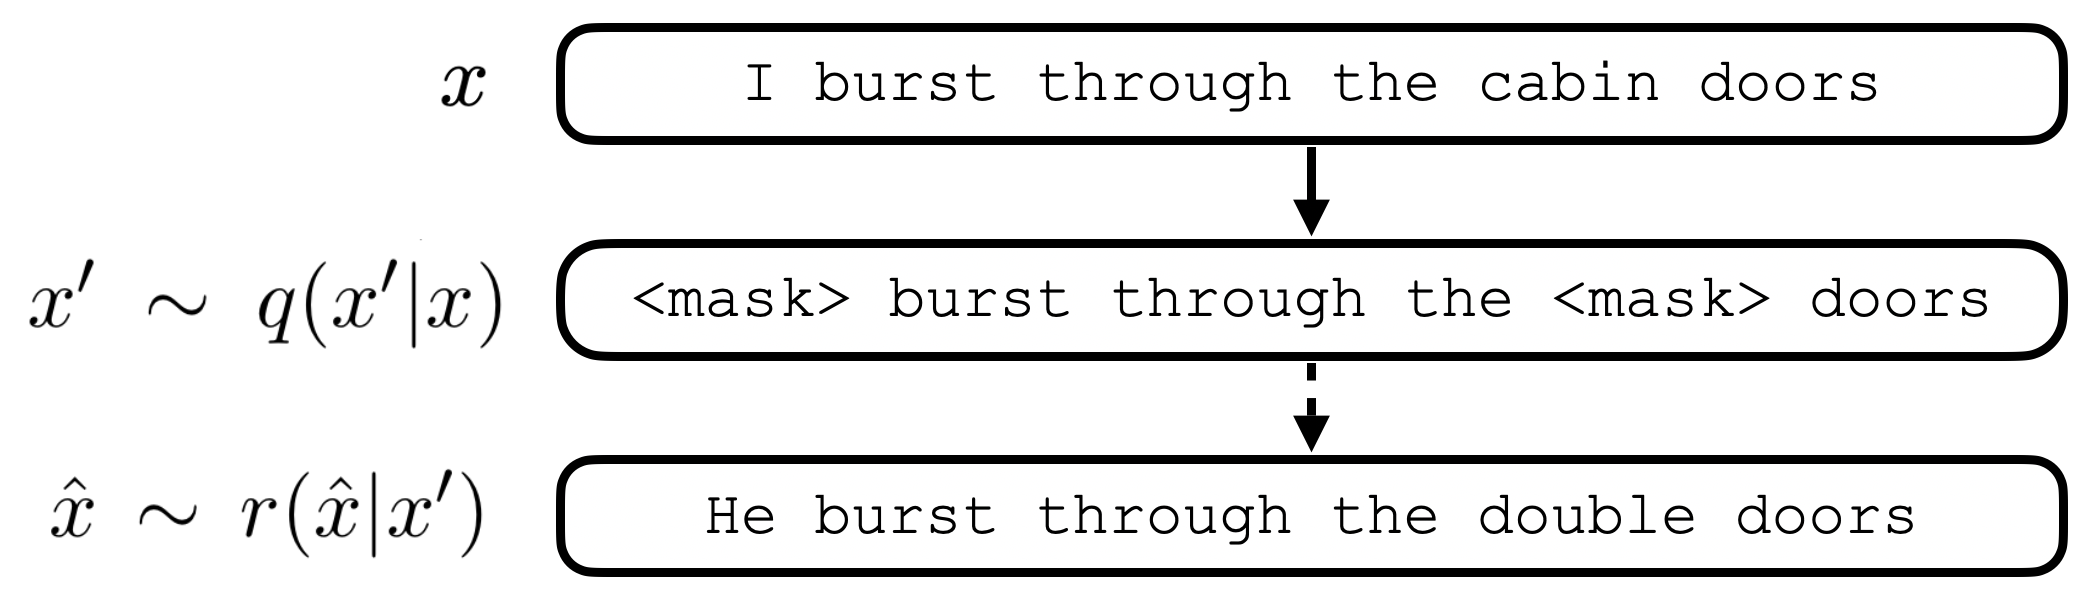
\includegraphics[scale=0.21]{img/bert_dae.png}
\caption{To sample from an MLM DAE, we apply the MLM corruption $q$ to the original sentence then reconstruct the corrupted sentence using our DAE $r$.}
\label{fig:dae_sampling}
\end{figure}

\subsection{Sampling from Denoising Autoencoders}
A denoising autoencoder (DAE) is an autoencoder trained to reconstruct a clean input $x$ from a stochastically corrupted one $x'\sim q(x'|x)$ by learning a conditional distribution $P_\theta (x| x')$ \citep{vincent2008extracting}.
We can sample from a DAE by successively corrupting and reconstructing an input using the following pseudo-Gibbs Markov chain: $x_t' \sim q(x'|x_{t-1})$, $x_t \sim P_\theta(x|x'_t).$
\comment{
\begin{align*}
    x_t' &\sim q(x'|x_{t-1})\\
    x_t &\sim P_\theta(x|x'_t) 
\end{align*}
}
As the number of training examples increases, the asymptotic distribution $\pi_n(x)$ of the generated samples approximate the true data-generating distribution $P(x)$ \citep{bengio2013generalized}.
This corruption-reconstruction process allows for sampling directly along the manifold that $P(x)$ concentrates on.

\subsection{Masked Language Models}
Recent advances in unsupervised representation learning for natural language have relied on pre-training models on a \textit{masked language modeling} (MLM) objective \citep{devlin2018, liu2019roberta}.
In the MLM objective, a percentage of the input tokens are randomly corrupted and the model is asked to reconstruct the original token given its left and right context in the corrupted sentence.
We use MLMs as DAEs \citep{lewis2019bart} to sample from the underlying natural language distribution by corrupting and reconstructing inputs (Figure \ref{fig:dae_sampling}).

% \section{Center Embedding Leads to The Hierarchical Rule}
\section{Data Complexity Determines Rule Preference}
\label{sec:data_complexity}

We find that models generalize hierarchically because they are trained on data which includes center embeddings, a linguistic structure which we describe in Section \ref{sec:center_embed}. Center-embedded sentences drive hierarchical generalization in both the QF task (Section \ref{sec:qf_result}) and the TI task (Section \ref{sec:ti_result}).

\begin{figure}[t!]
    \centering
    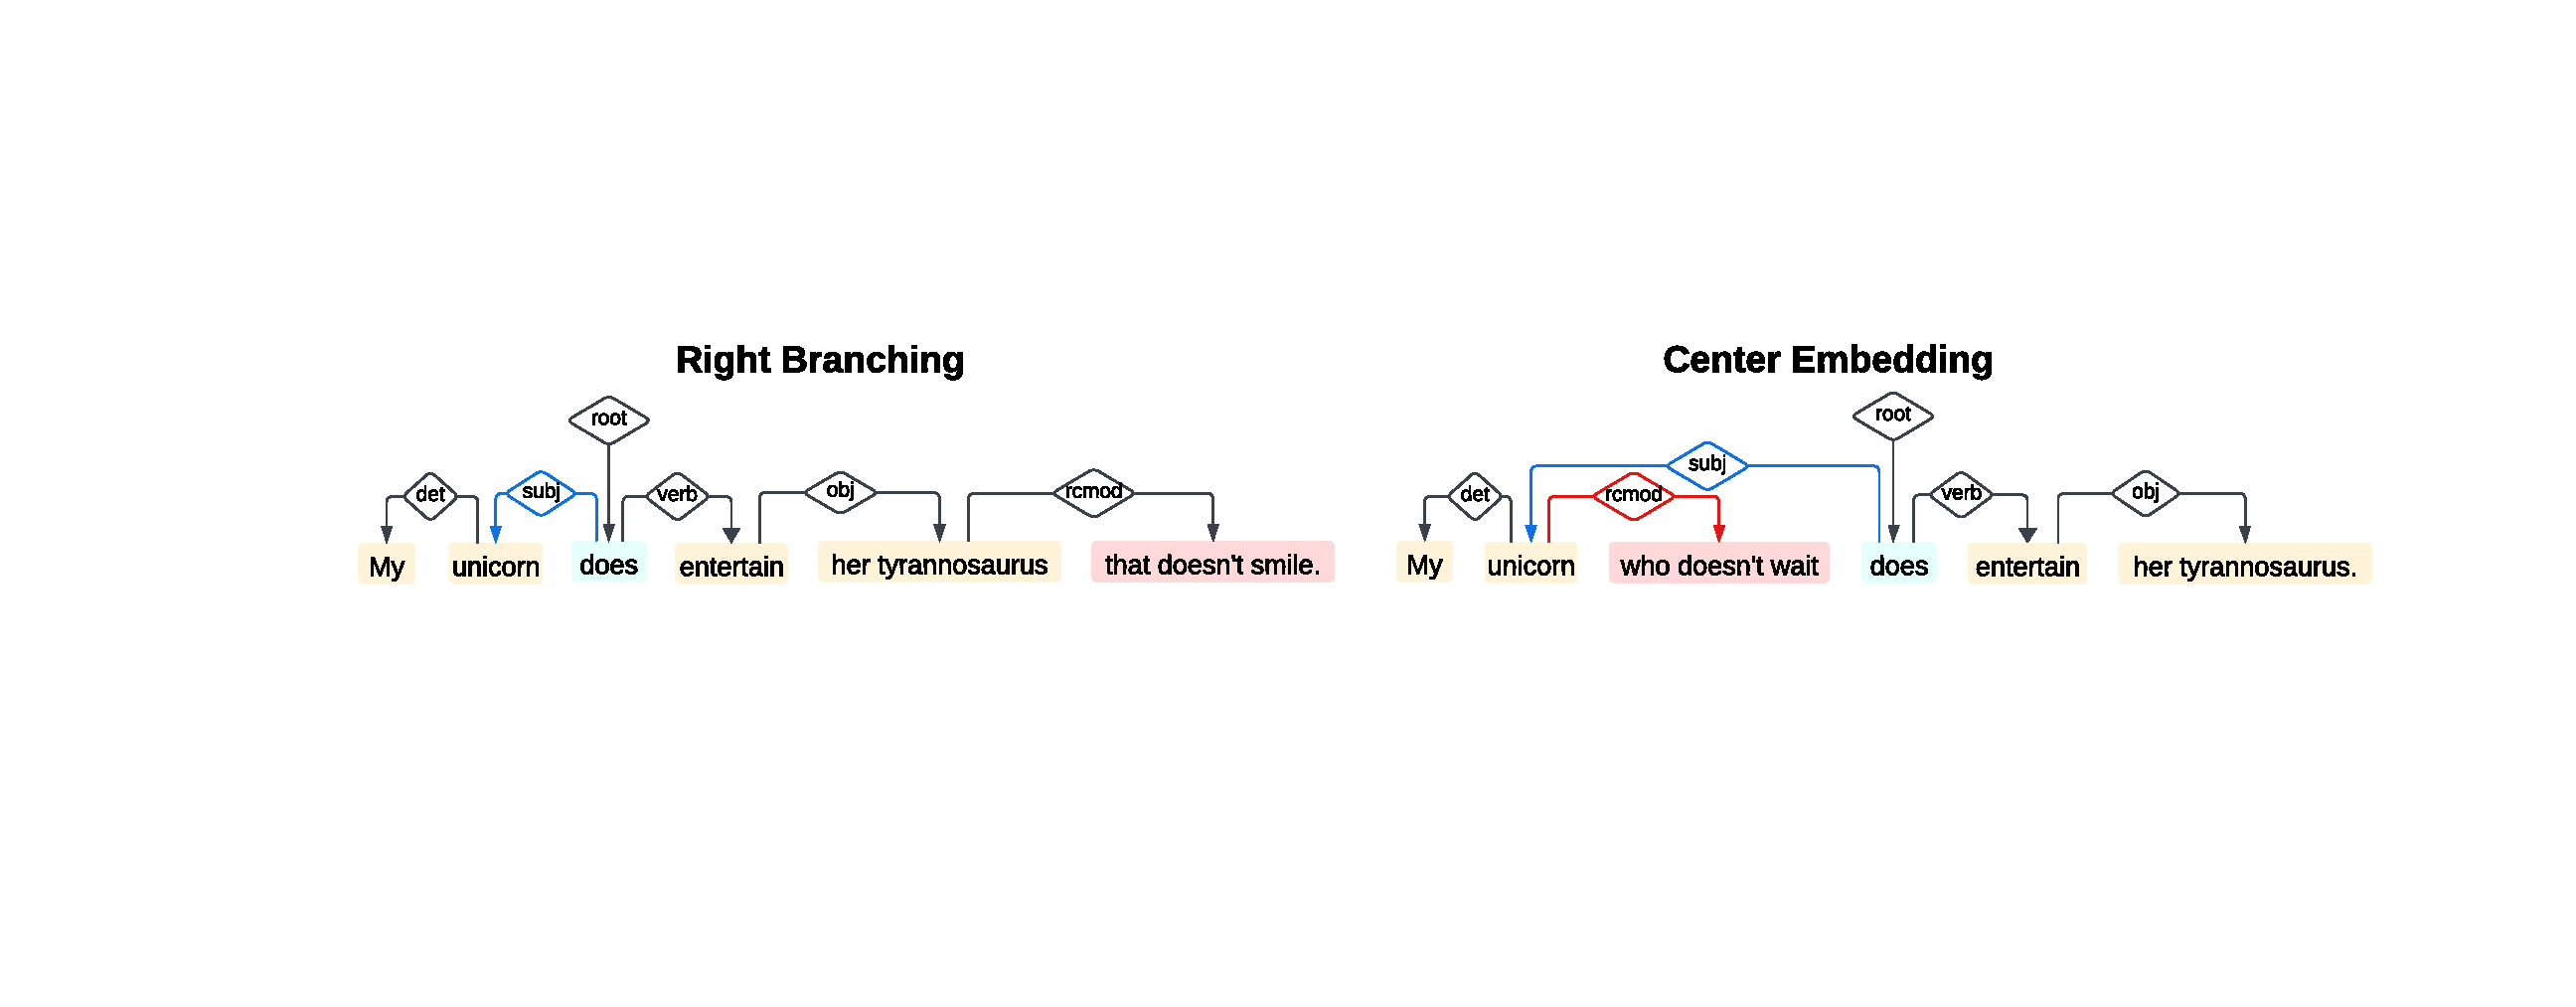
\includegraphics[width=1.0\textwidth]{figures/sentence_demo.pdf}
    \caption{\textbf{Sentence Examples.}   \textit{Left:} Right-branching sentence example. The linear progression of the main constituent is not interrupted by the relative clause. 
    \textit{Right:} Center-embedded sentence example. When the relative clause modifies the subject, it interrupts the linear progression of the main constituent. 
    }
    \label{fig:sentence_demo}
\end{figure}

\subsection{Center Embedding}
\label{sec:center_embed}
Center embedding occurs when a clause is placed recursively within another clause of the same type. Figure \ref{fig:sentence_demo} (\textit{left}) illustrates two examples of center-embedded sentences, where the embedded clause complicates syntactic parsing by placing an additional subject noun in between a verb and its own subject. Whereas center embeddings exhibit a recursive structure, sentences without center embeddings are exclusively right-branching. Right-branching structures may also include modifying clauses, but these clauses can only be appended at the end of the main clause, maintaining its linear flow (see Figure \ref{fig:sentence_demo}, \textit{right}). Linguists have long argued that center embeddings play a crucial role in grammar acquisition \citep{wexler1980formal} and give rise to tree-like syntactic structures \citep{Chomsky2015-bg}. 


We find that center embeddings, which are crucial for human language acquisition, also lead an LM to acquire hierarchical grammar rules. To correctly predict the next token, LMs must track syntactic connections between words in the context. In right-branching sentences, LMs can rely on linear proximity to identify these connections; as shown in Figure \ref{fig:sentence_demo}, a simple bigram model suffices to capture the subject-verb relationship for such sentences. In contrast, center embeddings introduce relative clauses of various lengths, making linear n-gram models inefficient for capturing subject-verb relationships. The recursive nature of the center embedding requires the model to track multiple subject-verb relationships: one for the main clause and a separate one for the embedded relative clause. In these cases, a tree structure is more efficient to model subject-verb relationships. 


\subsection{Question Formation Results}
\label{sec:qf_result}
As specified in Section \ref{sec:qf_task}, the training data for QF is ambiguous between the linear rule (i.e., moving the first auxiliary) and the hierarchical rule (i.e., moving the main auxiliary). Center-embedded sentences do not meet this ambiguity requirement and, therefore, cannot appear in question formation training samples. To ensure the model is exposed to diverse sentence types, \citet{McCoy2018-uv} introduced a secondary task to the QF training dataset: declaration copying. Like question formation, the declaration-copying example starts with a declarative sentence, but instead of transforming it, the model simply repeats it. Since the ambiguity requirement only applies to the primary question formation task, declaration-copying examples can include center embeddings. Concrete examples of both tasks can be found in Appendix \ref{appdx:data_sample}.


We train models on three modifications of the original training data, varying the composition of the declaration-copying subset. 
In \textit{Quest Only}, we remove all declaration-copying examples.
In \textit{Center embed}, we only keep center-embedded examples. In \textit{Right branch}, we only keep right-branching examples. 
Every modified training sets retains all examples of the primary task, question formation.
Every model trained, regardless of its training set composition, reaches 100\% in-distribution validation accuracy; however, the OOD generalization performance, shown in Figure \ref{fig:grokking_selection} (\textit{left}), differs significantly across the modified training sets. 

Our results confirm that declaration copying examples, specifically center embeddings, are essential for inducing hierarchical generalization.
Models trained without any declaration-copying examples fail to achieve an OOD accuracy above 75\%; so do models trained \textit{only} on right-branching  declaration-copying examples. When trained instead \textit{only} on center-embedded declaration-copying examples, models exhibit a strong preference for the hierarchical rule. This evidence suggests that center-embedded sentences direct a model towards the hierarchical rule. 

\begin{figure}[t!]
    \centering
    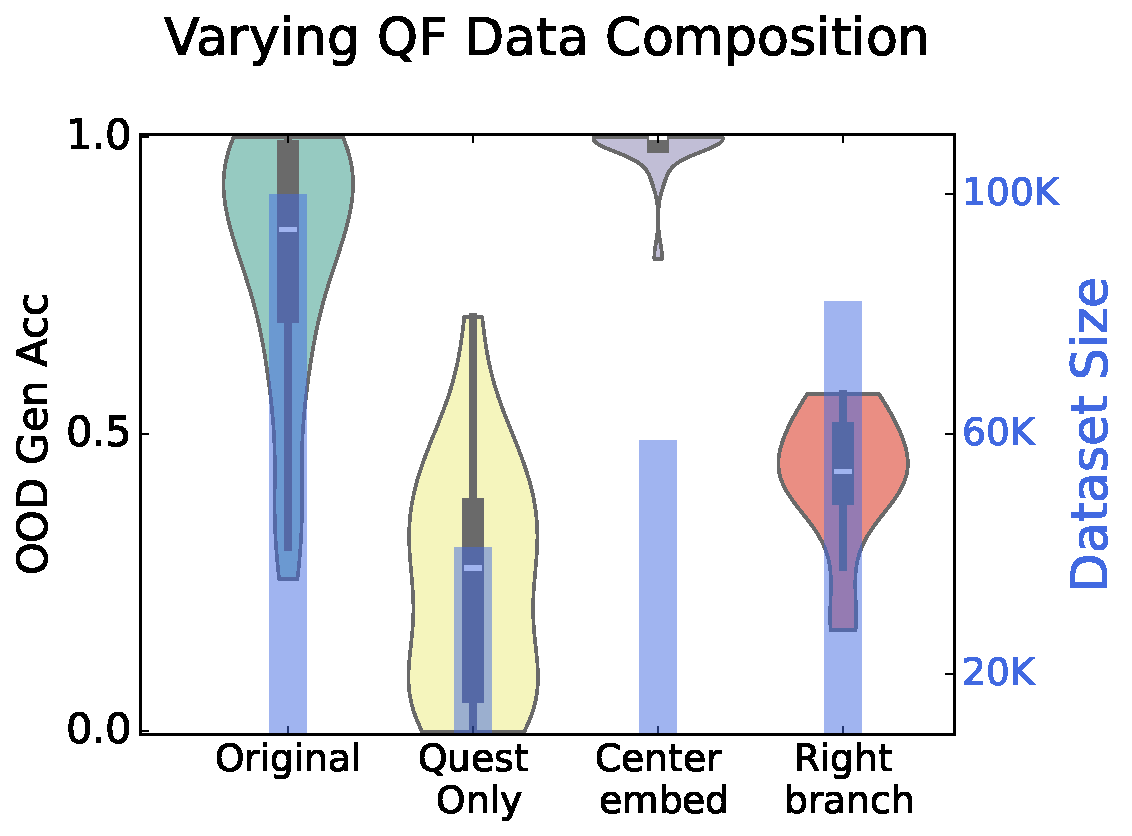
\includegraphics[width=0.41\linewidth]{figures/no_curriculum_main.pdf}
    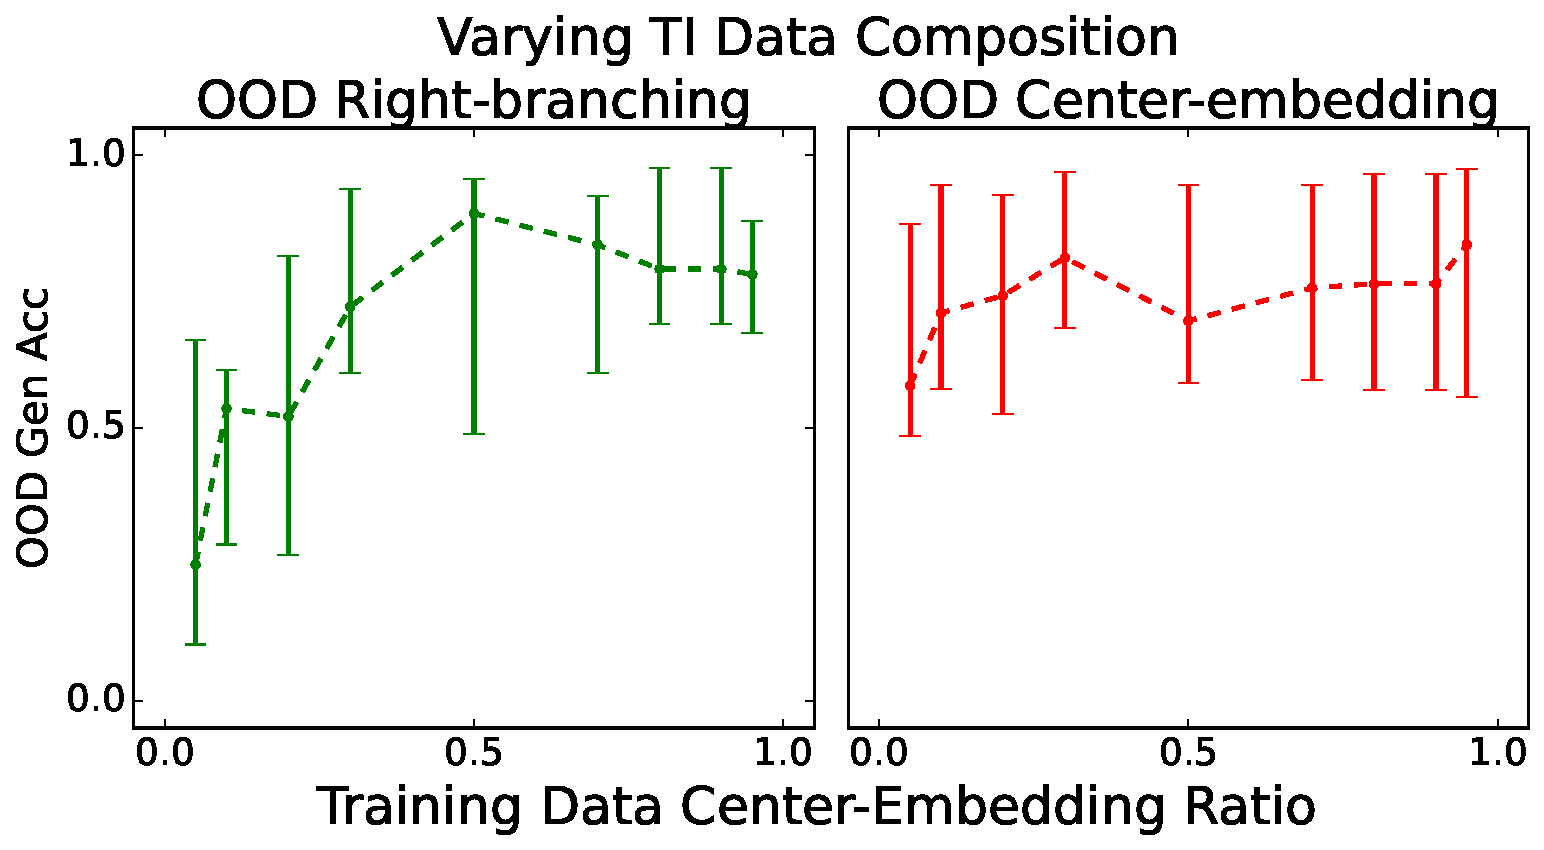
\includegraphics[width=0.55\linewidth]{figures/ti_simplicity_contamination.pdf}
    \caption{
    \textbf{Components of training data drive different generalization behaviors.} 
    \textit{Left:} Center-embedded sentences, which in the QF training data only appear in declaration copying examples, induce hierarchical generalization.
    \textit{Right:} Models are trained on different TI training data mixes and evaluated on two OOD sets: unambiguous right-branching sentences (\textit{green}) and unambiguous center-embedded sentences (\textit{red}). For center-embedded sentences, the hierarchical rule is preferred regardless of data mixes. For right-branching sentences, the model's preference for the hierarchical rule is exclusively driven by having a large mix of center-embedded sentences in the TI training data.}
    \label{fig:grokking_selection}
\end{figure}



\subsection{Tense Inflection Results}
\label{sec:ti_result}

In the TI training data, both right-branching and center-embedded sentences are made ambiguous by ensuring the distractor noun (i.e., a noun that appears between the main subject and the main verb) shares the same plurality as the main subject. For right-branching sentences, the distractor noun occurs in a prepositional phrase. For center-embedded sentences, the distractor noun occurs in a relative clause; either the subject or the object of the modifying clause can act as the distractor noun. We list examples below: 

\begin{enumerate}[itemsep=2pt,labelindent=10pt,topsep=0pt,parsep=0pt,partopsep=1pt, align=left, leftmargin=*]
    \item \textbf{Right Branching}: The noun in the prepositional phrase (e.g., `` \textit{to the cabinet}") acts as the distractor in the TI task.
    
    Example A (ID): \textit{The keys to the \textbf{cabinets} are on the table.}

    Example B (OOD): \textit{The keys to the \textbf{cabinet} are on the table.}
    
    \item \textbf{Center Embedding}: Either the subject or the object inside the relative clause acts as the distractor in the TI task.

    Example C (ID): \textit{The keys that unlock the \textbf{cabinets} are on the table.}

    Example D (OOD): \textit{The keys that unlock the \textbf{cabinet} are on the table.}
    
    
\end{enumerate}
We create variations of the TI training data by adjusting the ratio of right-branching to center-embedded samples while keeping the total training size constant.\footnote{The original training dataset contains a secondary past-tense copying task, to parallel the declaration-copying secondary task in QF. We show in Appendix \ref{appdx:ti_secondary} that the secondary task is not necessary, and we do not include it in our modified training sets.} A model's generalization behavior is tested on two OOD sets: one containing unambiguous right-branching sentences (e.g., Example B) and the other containing unambiguous center-embedded sentences (e.g., Example D). 

Generalization accuracies are shown in Figure \ref{fig:grokking_selection} (\textit{right}). When the training data is dominated by ambiguous right-branching sentences, the model fails to learn the hierarchical rule, as indicated by low OOD accuracy. However, when trained on a greater proportion of center-embedded sentences, the model systematically applies the hierarchical rule to both right-branching and center-embedded OOD sentences. As shown in Figure \ref{fig:grokking_selection} (\textit{right}), regardless of its training data mix, the model  generalizes hierarchically to OOD \textit{center embeddings}. In contrast, the model only generalizes hierarchically to \textit{right-branching sentences} after being exposed to a sufficient quantity of center-embedded sentences during training. In other words, the model eventually learns to treat non-recursive sequences as hierarchical through exposure to recursive center embeddings. These observations suggest that center embeddings drive the model's overall preference for tree structures. For further analysis of which center embedding structures induce this bias most efficiently, see Appendix \ref{appdx:obj_sbj_ctr_breakdown}.

% %%%%%%%%%%%%%%%%Previous version to preserve comments %%%%%%%%%%%%%%%%%%%%%%%%%%%%%%%%%%%%%%%%
% \iffalse
% \subsection{Tense Inflection} 
% \label{sec:ti_result}
% We now analyze hierarchical generalization in the tense inflection task, demonstrating the generality of our findings across grammatical rules. 
% The tense inflection setting from \citet{Linzen2016-vx} uses the same generation process as the question formation task, changing only the task itself.  
% This generation process leads to three types of sentences:

% \begin{enumerate}[itemsep=2pt,labelindent=10pt,topsep=0pt,parsep=0pt,partopsep=1pt, align=left, leftmargin=*]
%     \item The main verb immediately follows the subject noun.

%     Example: \textit{The keys are on the table.}
%     \item The main verb and the subject noun are separated by a prepositional phrase (e.g., `` \textit{to the cabinet}"). In all sentence examples, the prepositional phrase consistently follows the same syntactical structure and length (i.e., ``preposition $+$ determiner $+$ noun"). 

%     Example: \textit{The keys to the cabinet are on the table.}
%     \item The main verb and subject noun are separated by a relative clause, which can vary in syntactic composition and length.

%     Example: \textit{The keys that I used to unlock the cabinet are on the table.}
% \end{enumerate}


% By definition, both the first and second sentence types are right branching. In the second type, although a prepositional phrase is inserted within the main clause, it differs syntactically from a relative clause modifier. Unlike relative clause modifiers, prepositional phrases lack syntactic diversity, whereas relative clauses can exhibit the same of diversity as an entire sentence. In QF and TI data generated by CFG rules, a 4-gram model suffices to capture the subject-verb agreement. In contrast, relative clause modifiers (i.e., the third type) vary in both length and syntactic structure. All three sentence types are present in the original training data. Since sentences of the first type lack a distractor noun, they cannot be used to probe the model’s generalization, so the generalization set includes only the second and third types. As specified in Section \ref{sec:ti_task}, the TI training data only requires that the subject and distractor have the same plurality. Thus, center-embedded sentences can be included in the TI training data without violating the ambiguity requirement, and a secondary task is not necessary for TI.\footnote{In Appendix \ref{appdx:tense_tv}, we show that we can again leverage a secondary task such that a model trained on center-embedded tense inflection examples can generalize to right-branching sentences without having seen any examples of tense inflection on the sentence type, but not vice versa. }


% Our goal is to verify that center embeddings also drive OOD generalization in tense inflection. We create variations of the TI training data by adjusting the ratio of right-branching to center-embedded sentences, keeping the total training size constant. In Figure \ref{fig:ti_selection}, we report the model's OOD behavior across two data partitions. Figure \ref{fig:ti_selection} (\textit{left}) shows the model's generalization accuracy on unambiguous right-branching sentences when trained on different data mixes. When training data is dominated by ambiguous right-branching sentences, the model fails to learn the hierarchical rule, as indicated by low OOD generalization accuracy. However, as we increase the proportion of center-embedded sentences, these sentences---despite being ambiguous---bias the model towards the hierarchical rule, reflected by improved generalization accuracy.

% Figure \ref{fig:ti_selection} (\textit{right}) shows that the model consistently prefers the hierarchical rule for center-embedded sentences, regardless of data composition. These results indicate that the model’s preference for the hierarchical rule is primarily driven by center-embedded sentences. Moreover, with a high proportion of center-embedded sentences in the training data, this hierarchical rule preference extends to right-branching sentences as well.


% \fi
\section{Training Stabilizes if a Model Commits to a Rule}
\label{sec:stability}
Why do some runs fail to generalize hierarchically even when trained on hierarchy-inducing data? In this section, we will show that these failures are consequences of training instability; models only stabilize OOD if they commit to a general rule, whether it is the hierarchical or linear rule. Some random seeds fail to stabilize regardless of our training set composition.


\subsection{Instability During Training} 
\label{sec:tv_def}
When training models on both QF and TI tasks, some random seeds lead to highly unstable OOD behavior, with OOD generalization accuracy oscillating during training (see Appendix \ref{appdx:training_instabilty} for example training curves). We measure instability across training time using \textbf{total variation} (TV). Specifically, we checkpoint the model every 2K steps and measure the generalization accuracy $\mathrm{Acc}_t$ at each checkpoint timestep $t \in T$. The total variation is defined as: 
\begin{wrapfigure}[]{r}{0.4\textwidth}
    \centering
    \vspace{5mm}
    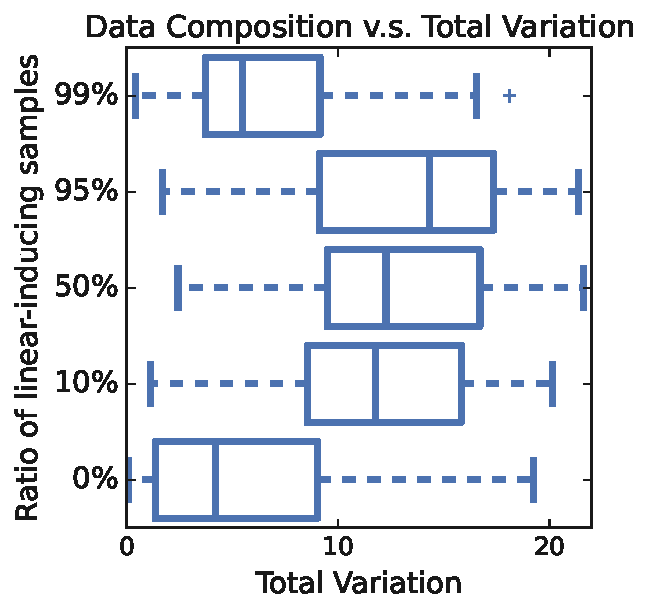
\includegraphics[width=0.85\linewidth]{figures/total_variation_box.pdf}
    \caption{\textbf{Training is unstable when different subsets of data compete.} Balanced mixtures of right-branching and center-embedded sentences have higher total variation than mixtures dominated by one or the other subset.}
    \vspace{-15mm}
    \label{fig:data_drives_inconsistency}
\end{wrapfigure}
\begin{align}
    \text{Total Variation (TV)} = 
    \frac{1}{|T|} \sum_{t \in T} 
    \left| \mathrm{Acc}_t - \mathrm{Acc}_{t-1} \right|
\end{align}

\subsection{Training Stability Ties to Rule Commitment}
\label{sec:intra_inter}

We now demonstrate that stable OOD behavior is associated with rule commitment. We construct QF training datasets with different proportions of hierarchy-inducing (i.e., center-embedded) and linearity-inducing (i.e., right-branching) declaration examples, while keeping all question examples from the original training set. Further details on the dataset can be found in Appendix~\ref{sec:simple_mixin}.


Figure \ref{fig:data_drives_inconsistency} shows the relationship between data homogeneity and training stability. When the training data is dominated by either linearity-inducing  (99\% linear) or hierarchy-inducing  (0\% linear) examples, more random seeds lead to stable OOD curves. When the training data is a heterogeneous mix instead, potential rules compete, leading to a higher proportion of unstable training runs.

By controlling for training instability, we reveal that generalization behavior is clustered and highly bimodal across random seeds. As shown in Figure \ref{fig:intra_inter_variance}, regardless of the data mix, the final generalization accuracy for all stable models is either $100\%$ or $0\%$---that is, stable models always commit to a systematic rule. 
While either rule can be implemented by a stable model, training data composition determines how likely a run is to stabilize in any rule and whether that rule is likely to be hierarchical or linear. 
Interestingly, when the data is heterogeneous (e.g., 10\% of examples are linearity-inducing right-branching sequences), the final generalization accuracy for stable runs is bimodally distributed, clustering around $100\%$ or $0\%$. 
 In fact, the horseshoe-shaped curves in Figure \ref{fig:intra_inter_variance} illustrate that the less stable a training run is, the less systematic the model tends to be in its OOD rules. 

\begin{figure}[t!]
    \centering
    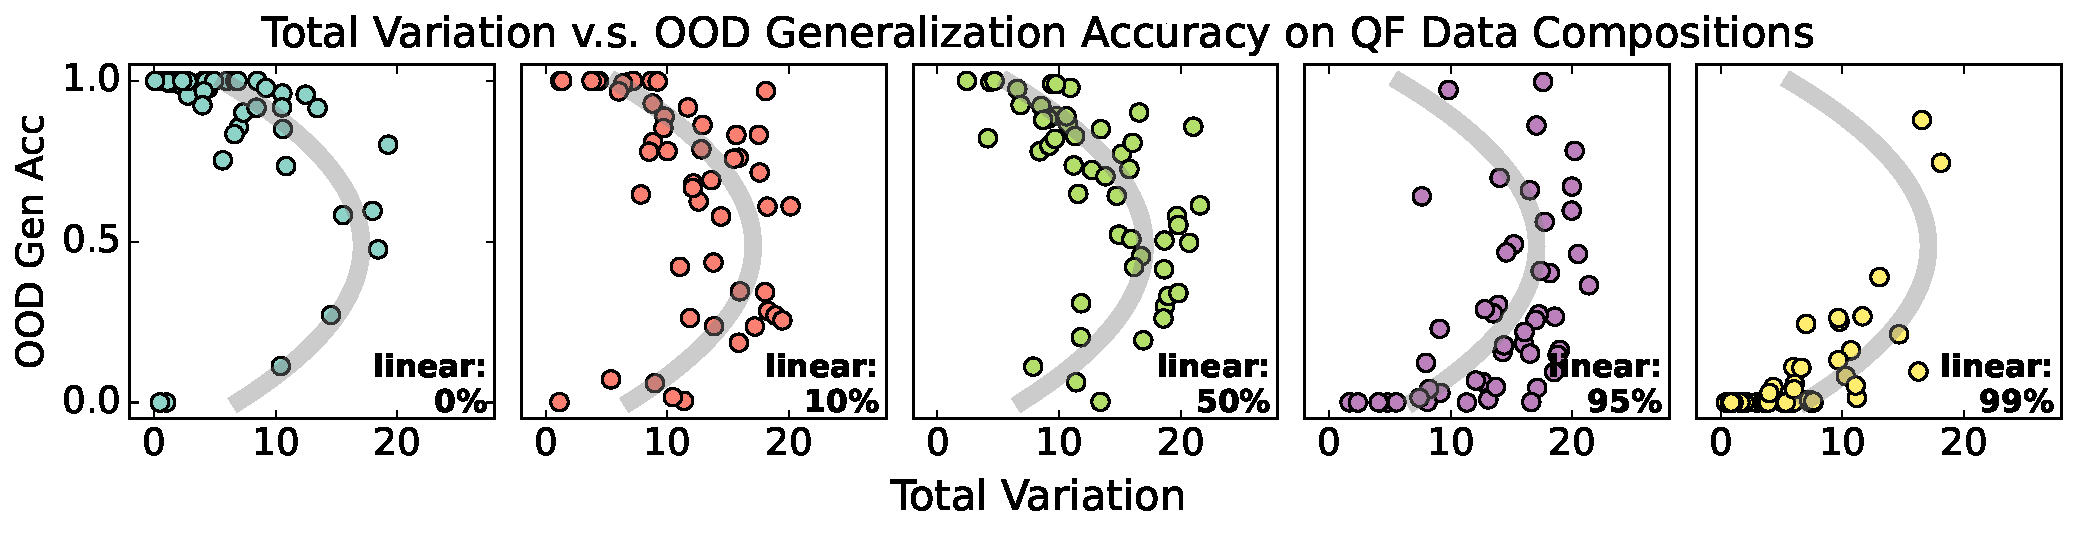
\includegraphics[width=1.0\linewidth]{figures/intra_inter_inconsistency_D270.pdf}
    \caption{\textbf{Training stability vs. final generalization accuracy for QF task.} OOD behavior stabilizes during training if a model commits to a general rule. By mixing data that induces the linear and hierarchical rules, we can create conditions that allow models to stabilize in either rule. ``Linear" denotes the proportion of linearity-inducing declarations in the data. 
    Grey line indicates the smoothed average curve across all five datasets.
    }
    \label{fig:intra_inter_variance}
    % \vspace{-5px}
\end{figure}

In summary, with heterogeneous training data, competition between rules leads to more unstable training runs. Even with heterogeneous data mixes, however, some runs can still stabilize if they  commit to one of the competing rules. Therefore, heterogeneous data also leads models to cluster into bimodally distributed OOD generalization accuracies, reflecting the distinct basins observed by \citet{Juneja2022-hj} in text classification.
Appendix \ref{appdx:tense_tv} presents similar findings for the TI task.


\section{Data Diversity Leads to Generalization}
\label{sec:data_diversity}
Our experiments thus far have linked training stability to rule commitment. In this section, we will show that models can, in fact, stabilize without a systematic rule---if they memorize their training instead. Less diverse training data produces models that stabilize through memorization, whereas more diverse training data produces models that commit to systematic rules. Furthermore, mirroring our previous findings in data complexity, intermediate levels of data diversity lead to highly unstable runs even when all examples induce the same rule. 
\subsection{Measuring Data Diversity}
\label{sec:data_diveristy}

We define the diversity of a dataset according to the syntactic similarity between different examples. 
We measure a sentence pair's similarity by the tree-edit distance (TED) of their latent tree representations \citep{Chomsky2015-bg}. When two sentences share the same syntax tree, transforming one into the other requires only leaf-node (i.e., vocabulary) changes. For example, \textit{My unicorn entertains her tyrannosaurus}, and, \textit{Your zebra eats some apples}, have different vocabulary but identical syntax trees. We define a dataset's diversity as the number of unique syntactic trees it contains. Similar methods are used to measure diversity in both natural language \citep{Huang2023-ab, Gao2024-fi, Ramirez2022-mx} and code \citep{Song2024-cg}. 

\subsection{Diversity and stability}
\label{sec:inverse}

We will next show that when the model is exposed to fewer unique syntax trees during training, it memorizes their patterns without reliably applying rules to unseen structures. We demonstrate the effect by designing datasets to induce either hierarchical or linear generalization and then adjusting adjusting the syntactic diversity of representative examples. Whichever rule is induced, diversity imposes three distinct regimes: stable memorization behavior at low diversity, stable generalization behavior at high diversity, and unstable behavior at intermediate levels. This transition, from stable to unstable to back to stable, forms a U-shaped curve of stability with respect to dataset diversity.

\paragraph{Hierarchy-inducing data}  
We first control data diversity on datasets that induce hierarchical generalization in QF. We construct variations of the QF training data with different levels of syntactic diversity. Each constructed training set includes 50K question samples and 50K center embedding declarations, while varying the syntactic diversity of the declaration examples. We train 50 random seeds for each modified training set and measure intra-run instability with total variation (see \ref{sec:tv_def}). To assess rule commitment, we report the proportion of runs achieving generalization accuracy either >95\% or < 5\%, indicating a commitment to either rule (here, hierarchical rule is preferred).


Figure \ref{fig:data_diversity_uscale} (\textit{left}) shows an inverse U-shaped relationship between data diversity and training instability, revealing three distinct regimes. Low-diversity data leads to the \textbf{memorization regime}, where training is stable but the model fails to commit to a rule. In Appendix \ref{appdx:memorizaition}, we confirm that models in this low-diversity regime apply the hierarchical rule to syntax structures memorized during training, but cannot extrapolate the rule to unseen  structures. High-diversity data leads to the \textbf{hierarchical generalization regime}, where training stabilizes because models commit to the hierarchical rule. In the mid-diversity \textbf{unstable regime}, the lack of data diversity hinders the likelihood of fully commiting to a rule but the data is too diverse to memorize easily. Overall, with insufficient diversity, relatively few runs learn to apply the hierarchical rule across all examples.

\paragraph{Linearity-inducing data} 
In Figure \ref{fig:intra_inter_variance} (\textit{right}), the model has a strong preference to apply the linear rule OOD when the training data contains 99\% linearity-inducing data (i.e., right branching sentences). However, Figure \ref{fig:grokking_selection} shows that when the training data contains \textit{exclusively} right-branching sentences, models do not consistently follow any systematic rule (further details in  Appendix \ref{sec:simple_mixin}). We can use data diversity to explain the failure to commit to a rule from exclusively right-branching examples: right-branching sentences lack syntactic variation, as the main auxiliary always follows the subject noun. This lack of syntax diversity prevents rule extrapolation. By introducing center embeddings in just 1\% of sentences, we introduce the diversity necessary to learn a systematic generalization rule. 

To confirm that data diversity is also key to rule commitment for when data is mostly linearity-inducing, we create variations of QF training data with 50K questions and 50K declarations, including 99\% right-branching and 1\% center-embedded sentences. We control the diversity of \textit{center-embedded} sentences as before and use the proportion of runs achieving generalization accuracy either above 95\% or below 5\% to quantify the likelihood of committing to any rule (in this data setting, linear rule is preferred). Figure \ref{fig:data_diversity_uscale} (\textit{right}) shows that training is least stable at intermediate levels of diversity, again providing three regimes: the memorization, unstable, and \textbf{linear generalization regime}.


\begin{figure}[t]
    \centering
    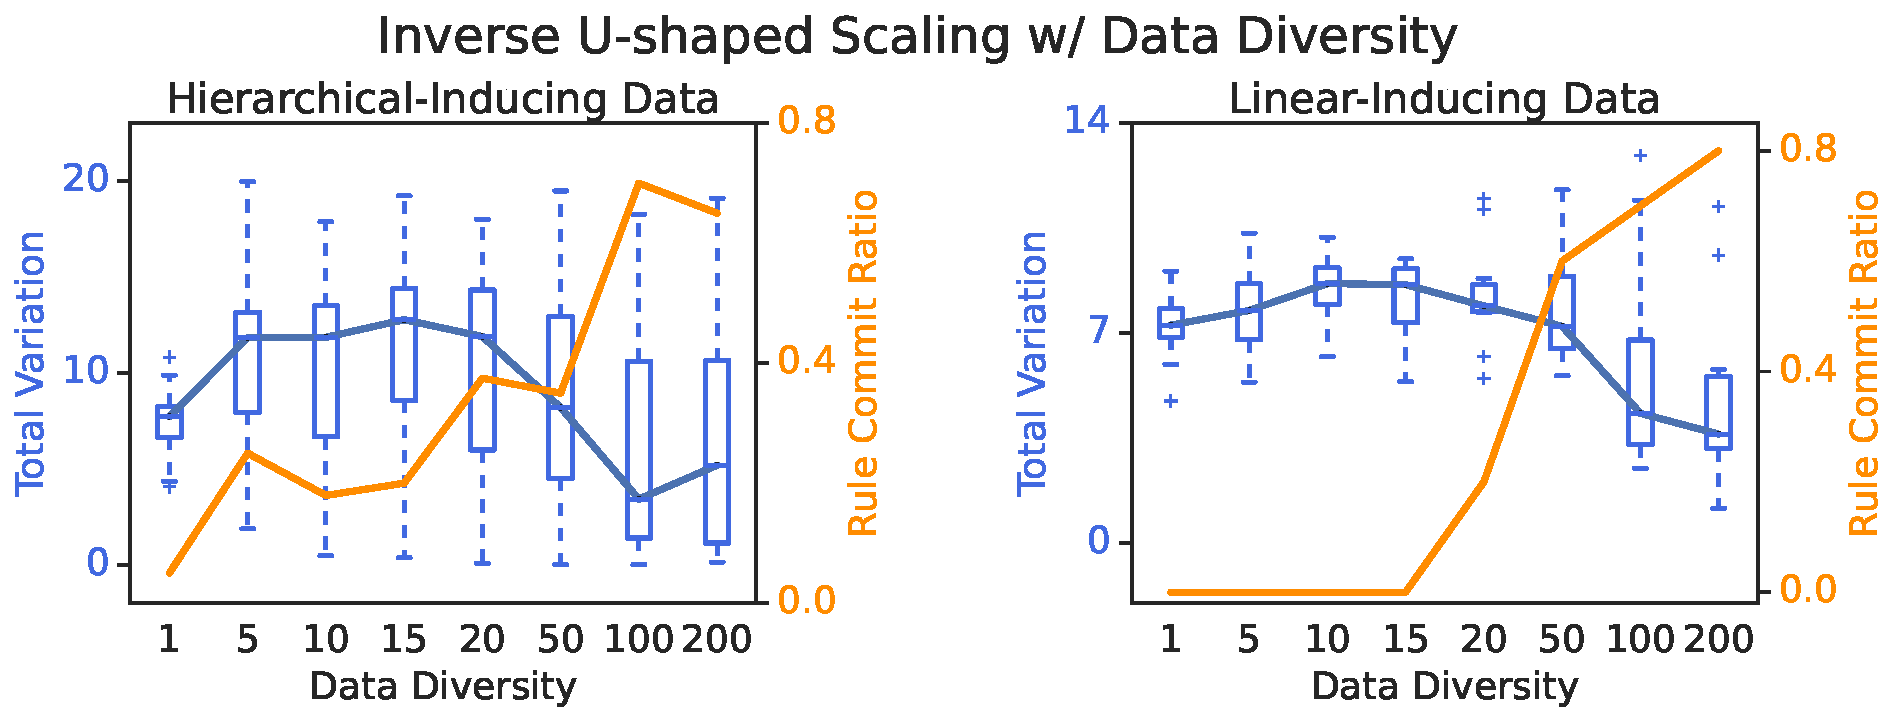
\includegraphics[width=0.8\linewidth]{figures/data_diversity_uscale.pdf}
    \caption{\textbf{Inverse U-shaped relationship between training stability and data diversity.} Whether training data favors the hierarchical (\textit{left}) or linear (\textit{right}) rule, diverse data promotes systematic rules over example memorization. At low diversity, training is stable but the model memorizes individual syntactic patterns rather than committing to a rule. With moderate data diversity, training becomes unstable. As diversity increases further, the model commits to a rule and training is the most stable.} 
    \label{fig:data_diversity_uscale}
    \vspace{-4px}
\end{figure}

Hyperbolic embeddings embed hierarchical information with high
fidelity and few dimensions. We explored the limits of this approach
by describing scalable, high quality algorithms. We hope the
techniques here encourage more follow-on work on the exciting
techniques of \citet{fb, ucl}. As future work, we hope to explore how
hyperbolic embeddings can be most effectively incorporated into downstream
tasks and applications.

% % \clearpage
\section*{Ethics Statement}
This research does not present any direct ethical concerns. The work involves empirical studies of machine learning models and their behavior in language tasks. No human subjects, sensitive data, or high-stakes applications were involved in this research. Therefore, no specific ethical considerations were necessary for this work.
\section*{Reproducibility Statement}
All relevant details regarding the experimental setup including model architecture, hyperparameters, and data preprocessing, are included in the main text (Section \ref{sec:model_and_training}) and appendices (Section \ref{sec:simple_mixin}).  Additionally, the code and scripts used to run the experiments are provided in the supplementary material and will be made publicly available upon acceptance.
\section*{Acknowledgments}
Tian Qin and David Alvarez-Melis were partially supported by the Kempner Institute, the Aramont Fellowship Fund, and the FAS Dean’s Competitive Fund for Promising Scholarship. We are very grateful to David Chiang, Isabel Papadimitriou, Ekdeep Singh, John Rawski, Will Merrill for their valuable feedback and discussions that helped improve this work. 
\clearpage
%\clearpage
% \vskip 0.2in
% \bibliography{paperpile}
% \bibliographystyle{iclr2024_conference}
% \setlength\bibitemsep{0.5\itemsep}
% \ifcompressbib
% \renewcommand*{\bibfont}{\footnotesize}
% \fi
\newrefcontext[sorting=nyt]
\printbibliography[title=References]
% \bibliography{paperpile,iclr2025_conference}
% \bibliographystyle{iclr2025_conference}

\clearpage
\appendix

% 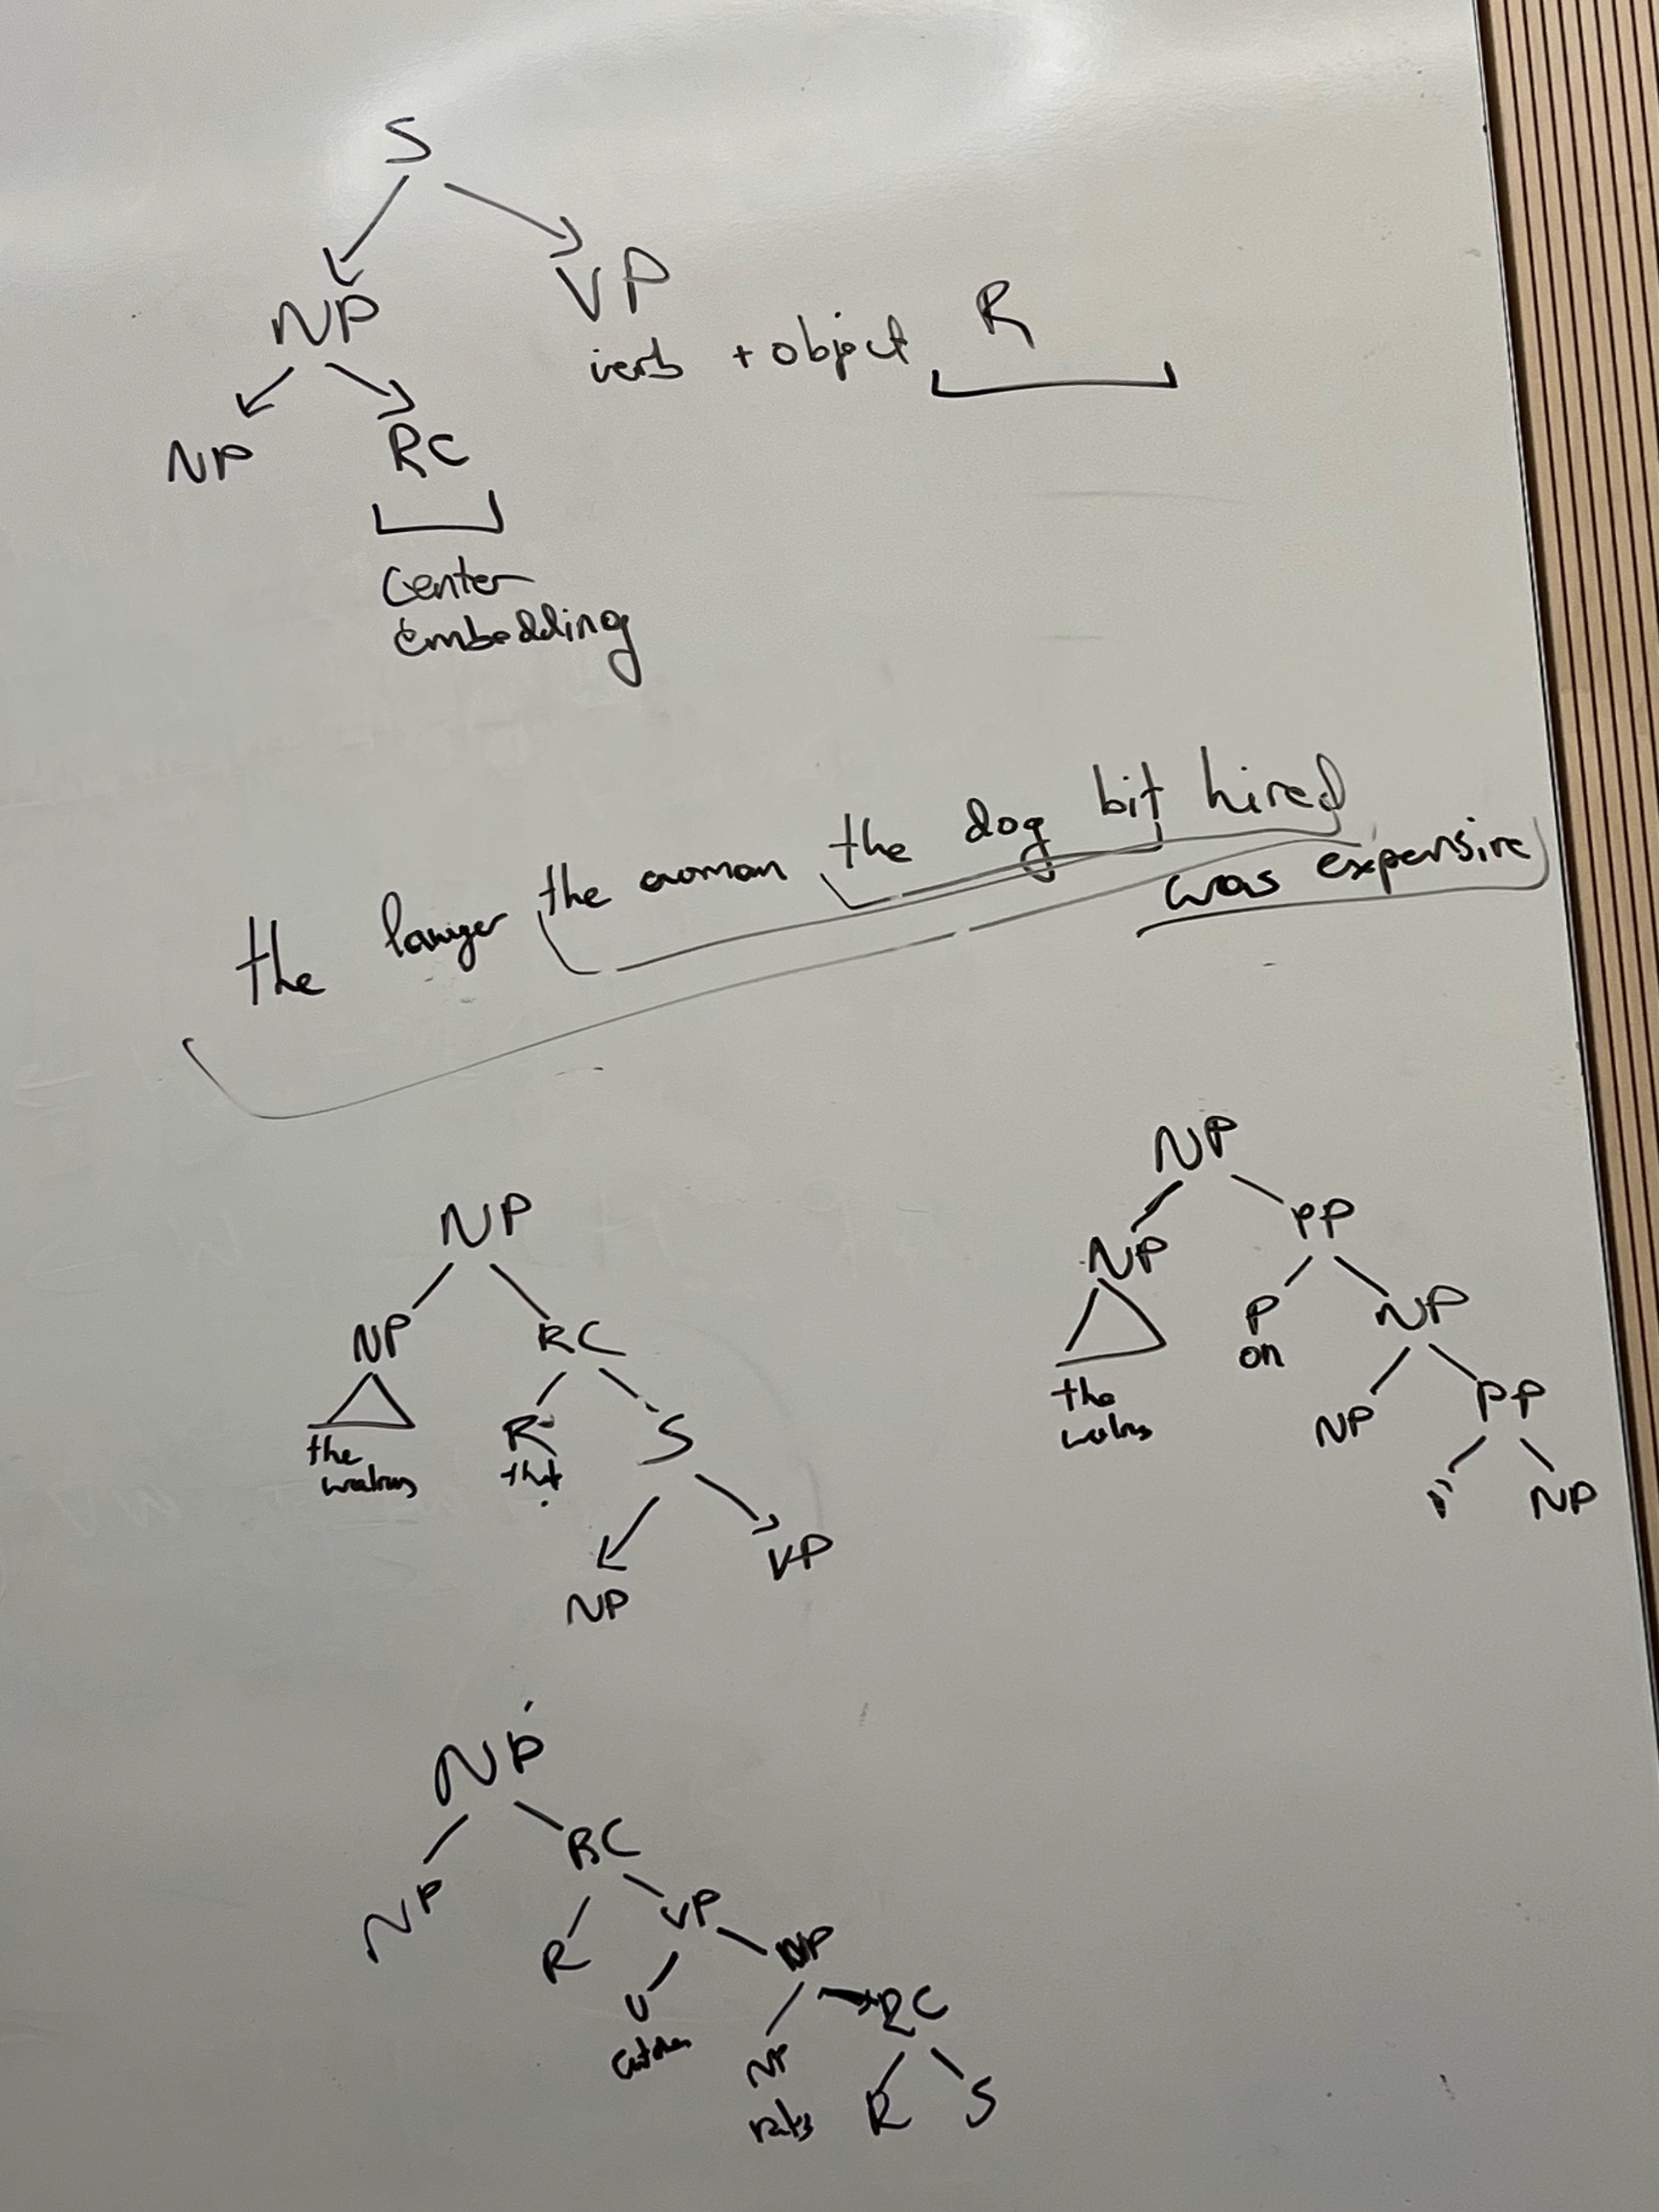
\includegraphics[width=0.48\textwidth]{figures/center_embed_demo.jpeg}


% \includegraphics[width=1.0\textwidth]{figures/test_acc_analysis_D280_52714736.png}
% \includegraphics[width=1.0\textwidth]{figures/test_acc_analysis_D281_52716914.png}
% \includegraphics[width=1.0\textwidth]{figures/test_acc_analysis_D283_52717479.png}
% \includegraphics[width=1.0\textwidth]{figures/test_acc_analysis_D284_52695892.png}

% Oct 23 Meeting updates:
% \begin{enumerate}
%     \item Question Formation:
%     \begin{enumerate}
%         \item Train only on center-embded decl leads to very consistent generalization
%         \item Unexpected: We initially suspect that we can introduce center-embeded decl in the question formation task, and thus get rid of the auxiliary task. But it turns out not to be the case. Model NEEDs to seem examples where the first auxiliary and the main auxiliary differ.
%         \item memorization: see appendix
%     \end{enumerate}
%     \item  Tense Inflection:
%     \begin{enumerate}
%         \item Now switch to a new way of presenting: (1) show that center-emebded sentences generalize hierarchically (2) Show that right-branching sentences don't. (3) Finally, show that with sufficient amount of center-embeded sentences, right-branching sentences can also generalize hieratically. Furthermore, the use of auxiliary task facilitate sentence type OOD generalization 
%         \item Looked into the evaluation objective - the default one, even though it is slightly weird is consistent with some other alternatives I tried. 
%     \end{enumerate}
%     \item Figure 1 alternative version. 
% \end{enumerate}


\section{Related Work Extended}
\label{appdx:related}
\subsection{Syntax and Hierarchical Generalization}
While works mentioned in Section \ref{sec:syntax_related} focused on models trained from scratch, another line of research examined the inductive bias of pretrained models. \citet{Mueller2024-qz, Mueller2023-xq} pretrained transformers on text corpora such as Wikipedia and CHILDES \citep{MacWhinney2014-jq} before fine-tuning them on the question formation task. They found that exposure to large amounts of natural language data enables transformers to generalize hierarchically.


Instead of using the question formation task as a probe, \citet{Hewitt2019-fc, Murty2022-lw} directly interpreted model's internal representation to understand whether transformers constrain their computations to to follow tree-structure patterns. \citet{Hewitt2019-fc} demonstrated that the syntax tress are embedded in model's representation space. Similarly, \citet{Murty2022-lw} projects transformers into a tree-structured network, and showed that transformers become more tree-like over the course of training on language data. 

\citet{Papadimitriou2023-gj, Papadimitriou2020-la} and \citet{Mueller2022-rm} also studied how pretraining data could introduce an inductive bias in language acquisition. \citet{Papadimitriou2023-gj} specifically identified that by pretraining models on data with a recursive structure  their performance when later finetuning them on natural language. This finding is closely related to our conclusions around the importance of recursive center embeddings. 



% \paragraph{Random variation} 
\subsection{Random Variation}
Specific training choices, such as hyperparameters, are crucial to model outcomes. However, even when controlling for these factors, training machine learning models remains inherently stochastic—models can be sensitive to random initialization and the order of training examples. \citet{Zhou2020-xt, D-Amour2022-tl, Naik2018-og} reported significant performance differences across model checkpoints on various analysis and stress test sets. \citet{Zhou2020-xt} further found that instability extends throughout the training curve, not just in final outcomes. To investigate the source of this inconsistency, \citet{Dodge2020-pb} compared the effects of weight initialization and data order, concluding that both factors contribute equally to variations in out-of-sample performance.


Similarly, \citet{Sellam2021-rz} found that repeating the pre-training process on BERT models can result in significantly different performances on downstream tasks. To promote more robust experimental testing, they introduced a set of 25 BERT-BASE checkpoints to ensure that experimental conclusions are not influenced by artifacts, such as specific instances of the model. In this work, we also observe training inconsistencies across runs on OOD data, both during training and at convergence. Unlike prior studies that focus on implications of random variations on experimental design, we study the source of training inconsistencies and link these inconsistencies to simplicity bias and the characteristics of the training data.



% \paragraph{Simplicity bias} 
\subsection{Simplicity Bias}
Models often favor simpler functions early in training, a phenomenon known as simplicity bias \citep{Hermann2020-ja}, which is also common in LMs. \citet{Choshen2022-qj} found that early LMs behave like n-gram models, and \citet{Saphra2019-sq} observed that early LMs learn simplified versions of the language modeling task. \citet{McCoy2019-br} showed that even fully trained models can rely on simple heuristics, like lexical overlap, to perform well on Natural Language Inference (NLI) tasks. \citet{Chen2023-fi} further explored the connection between training dynamics and simplicity bias, showing that simpler functions learned early on can continue to influence fully trained models, and mitigating this bias can have long-term effects on training outcomes.


Phase transitions have been identified as markers of shifts from simplistic heuristics to more complex model behavior, often triggered by the amount of training data or model size. In language models, \citet{Olsson2022-ed} showed that the emergence of induction heads in autoregressive models is linked to handling longer context sizes and in-context learning. Similar phase transitions have been studied in non-language domains, such as algorithmic tasks \citep{Power2022-hz, Merrill2023-an} and arithmetic tasks \citep{Nanda2023-zm, Barak2022-ub}.


In the context of hierarchical generalization, \citet{Ahuja2024-ul} used a Bayesian approach to analyze the simplicity of hierarchical versus linear rules in modeling English syntax. They argued that transformers favor the hierarchical rule because it is simpler than the linear rule. However, their model fails to explain (1) why learning the hierarchical rule is delayed (i.e., after learning the linear rule) and (2) why hierarchical generalization is inconsistent across runs. In this work, we offer a different perspective, showing that a model's simplicity bias towards either rule is driven by the characteristics of the training data.


\appendix

% \section{Claimed Emergent Abilities}
% \label{app:claimed_emergent_abilities}

% We compile the models, tasks and metrics that different papers have claimed reveal emergent abilities of large language models. This list may be incomplete or inaccurate, but represents a good faith attempt to compile this information. Note: quantifying model scale when an ability emerges is complicated by the fact that different papers report model scale differently, either as (a) number of parameters \cite{brown2020language, ganguli2022predictability}, (b) effective number of parameters \cite{srivastava2022beyond} or (c) training FLOPs \cite{wei2022emergent}.

% \begin{table}[h!]
%     \centering
%     \begin{tabular}{|l|c|c|c|}
%     \hline
%         Task & Model Families & Metric & Model Scale at Emergence \\
%         \hline
%         2-Digit Addition \cite{brown2020language} & GPT-3 & Accuracy & 13B Parameters\\
%         2-Digit Subtraction \cite{brown2020language} & GPT-3 & Accuracy & 13B Parameters\\
%         3-Digit Addition \cite{brown2020language, ganguli2022predictability} & GPT-3 & Accuracy & 175B Parameters\\
%         3-Digit Subtraction \cite{brown2020language} & GPT-3 & Accuracy & 175B Parameters\\
%         MMLU \cite{ganguli2022predictability} & GPT-3, Gopher & Accuracy & 200B, 300B Parameters\\
%         Program Synthesis \cite{ganguli2022predictability} & Google Internal & \% Samples Solving Task & 200B Parameters\\
%         Figure of Speech Detection \cite{srivastava2022beyond} & ? & ? & $\sim 10^{11}$ Effective Parameters \\
%         IPA Transliterate \cite{srivastava2022beyond, wei2022emergent} & LaMDA, GPT-3 & BLEU & $\sim 10^{23}, \sim 10^{23}$ Training FLOPs\\
%         Periodic Elements \cite{srivastava2022beyond} & ? & ? & ?\\
%         Modified Arithmetic \cite{srivastava2022beyond, wei2022emergent} & GPT-3, LaMDA & Accuracy & $\sim 10^{23}, \sim 10^{24}$ Training FLOPs\\
%         Repeat Copy Logic \cite{srivastava2022beyond} & ? & ? & $10^{11}$ Effective Parameters\\
%         Word Unscrambling \cite{srivastava2022beyond, wei2022emergent} & LaMDA & Exact Match & $\sim 10^{24}$ Training FLOPs\\
%         Persian QA \cite{wei2022emergent} & PaLM & Exact Match & $\sim 10^{24}$ Training FLOPs\\
%         Truthful QA \cite{wei2022emergent} & Gopher & Accuracy & $\sim 10^{23}$ Training FLOPs\\
%         Grounded Mappings \cite{wei2022emergent} & ? & ? & ?\\
%         Multi-task NLU \cite{wei2022emergent} & ? & ? & ?\\
%         Word in context \cite{wei2022emergent} & ? & ? & $\sim 10^{24}$ Training FLOPs\\
%         \hline
%     \end{tabular}
%     \newline
%     \caption{\textbf{Tasks, model families, metrics and number of parameters for emergent abilities.}}
%     \label{tab:my_label}
% \end{table}


% \section{Exponentiated Negative Cross Entropy Lower Bounds Accuracy}
% \label{app:acc_bound}

% Consider batch size $B$ with length $L$. During training i.e. with teacher-forcing, the per-token accuracy (averaged over batch index $b$ and sequence index $l$) is defined as:
% %
% \begin{align}
%     \text{Acc} &\defeq \frac{1}{B} \sum_b \frac{1}{L} \sum_l p(t_{bl}^* | t_{b, <l}^*)\\
%     &= \frac{1}{BL} \sum_{b, l} p(t_{bl}^* | t_{b, <l}^*)
% \end{align}

% The cross entropy (commonly averaged over the batch) is defined as:
% %
% \begin{align}
%     \mathcal{L}_{CE} &\defeq -\frac{1}{B} \sum_b \log p(t_{b 1}^*, ..., t_{b L}^*)\\
%     &= -\frac{1}{B} \sum_b \log \prod_l p(t_{b l}^*| t_{b, <l}^*)\\
%     &= -\frac{1}{B} \sum_{b, l} \log p(t_{bl}^* | t_{b, <l}^*)
% \end{align}

% To make the comparison between accuracy and cross entropy a little easier, let's normalize the cross entropy by the sequence length:
% %
% \begin{align}
%     \mathcal{L}_{CE/L} &\defeq \frac{1}{L}\mathcal{L}_{CE}\\
%     &=  -\frac{1}{BL} \sum_{b, l} \log p(t_{bl}^* | t_{b, <l}^*)
% \end{align}

% Recall that Jensen's inequality tells us that for any random variable $X$, $\log \mathbb{E}[X] \geq \mathbb{E}[\log X]$. The relationship between sequence-length-normalized cross entropy and accuracy is thus:
% %
% \begin{align}
%     -\mathcal{L}_{CE/L} = \frac{1}{BL} \sum_{b, l} \log p(t_{bl}^* | t_{b <l}^*) &\leq \log \frac{1}{BL} \sum_{b, l}  p(t_{bl}^* | t_{b <l}^*) = \log \text{Acc}\\
%     \exp(- \mathcal{L}_{CE/L}) &\leq \text{Acc}
% \end{align}

% Consequently, we see that driving the cross entropy loss to $0$ necessarily drives the accuracy to $1$.

% TODO: Can we use the second moment method to derive bounds on how (un)likely a subset of tokens are to deviate from the mean?


\section{Approximate Behavior of Metrics on Sequential Data}
\label{app:metric_scaling}

How do different metrics behave when used to measure autoregressive model outputs? Precisely answering this question is tricky and possibly analytically unsolvable, so we provide an approximate answer here.

Notationally, we consider $N$ test data of length $L$ (here, length is measured in tokens) with targets denoted $t_n \defeq (t_{n1}, t_{n2}, ... t_{nL})$, the autoregressive model has a true-but-unknown per-token error probability of $\epsilon \in [0, 1]$ and the model outputs prediction $\hat{t}_n \defeq (\hat{t}_{n1}, \hat{t}_{n2}, ... \hat{t}_{nL})$. This assumes that the model's per-token error probability is constant, which is empirically false, but modeling the complex dependencies of errors is beyond our scope.

\subsection{Per-Token Error Probability is Resolution-Limited}
\label{app:metric_scaling:resolution_limited}

Note that because we have $N$ test data, each of length $L$, our resolution for viewing the per-token error probability $\epsilon$ is limited by $1/NL$. 
Here, resolution refers to ``the smallest interval measurable by a scientific instrument; the resolving power."
To explain what resolution means via an example, suppose one wants to measure a coin's probability of yielding heads.
After a single coin flip, only two outcomes are possible (H, T), so the resolution-limited probability of heads is either $0$ or $1$.
After two coin flips, four outcomes are possible (HH, HT, TH, TT), so the resolution-limited probability of heads is now one of $0, 0.5, 1$.
After $F$ coin flips, we can only resolve the coin's probability of yielding heads up to $1/F$.
Consequently, we introduce a resolution-limited notation:
%
\begin{equation}
    \nint{a}_b \defeq \text{$a$ rounded to the nearest integer multiple of $1/b$}
\end{equation}

\subsection{Token Edit Distance}
\label{app:metric_scaling:token_edit_distance}

We first consider an adaptation of the Levenshtein (string edit) distance for models that function on tokens rather than characters, an adaptation we term the \textit{token edit distance}. The token edit distance between two token sequences $t_n, \hat{t_n}$ is defined as the integer number of additions, deletions or substitutions necessary to transform $t_n$ into $\hat{t}_n$ (or vice versa).

\begin{align}
    \text{Token Edit Distance}(t_n, \hat{t}_n)  &\defeq \text{Num Substitutions} + \text{Num. Additions} + \text{Num. Deletions}\\
    &= \sum_{\ell =1}^L \mathbb{I}[t_{n\ell} \neq \hat{t}_{n\ell}] + \text{Num. Additions} + \text{Num. Deletions}\\
    &\geq \sum_{\ell =1}^L \mathbb{I}[t_{n\ell} \neq \hat{t}_{n\ell}]
\end{align}

The expected token edit distance is therefore:

\begin{align}
    \mathbb{E}[\text{Token Edit Distance}(t_n, \hat{t}_n)] &\geq \mathbb{E}[\sum_{\ell =1}^L \mathbb{I}[t_{n\ell} \neq \hat{t}_{n\ell}]]\\
    &= \sum_{\ell =1}^L p(t_{n\ell} \neq \hat{t}_{n\ell})\\
    &\approx L (1 - \epsilon)
\end{align}

The resolution-limited expected token edit distance is therefore:

\begin{equation}
    \nint{\mathbb{E}[\text{Token Edit Distance}(t_n, \hat{t}_n)]}_{NL} \geq L \Big(1 - \nint{\epsilon}_{NL} \Big)
\end{equation}

From this, we see that the expected token edit distance scales approximately linearly with the resolution-limited per-token probability. The real rate is slightly higher than linear because additions and deletions contribute an additional non-negative cost, but modeling this requires a model of how likely the model is to overproduce or underproduce tokens, which is something we do not currently possess.

\subsection{Accuracy}
\label{app:metric_scaling:accuracy}

\begin{align}
    \text{Accuracy}(t_n, \hat{t}_n) &\defeq \mathbb{I}[\text{No additions}] \, \mathbb{I}[\text{No deletions}] \, \prod_{l=1}^L \mathbb{I}[t_{nl} = \hat{t}_{nl}]\\
    &\approx \prod_{l=1}^L \mathbb{I}[t_{nl} = \hat{t}_{nl}]
\end{align}

As with the Token Edit Distance (App. \ref{app:metric_scaling:accuracy}), we ignore how likely the language model is to overproduce or underproduce tokens because we do not have a good model of this process. Continuing along,

\begin{align}
    \mathbb{E}[\log \text{Accuracy}] &= \sum_l \mathbb{E}[\log \mathbb{I}[t_{nl} = \hat{t}_{nl}]]\\
    &\leq \sum_l \log \mathbb{E}[\mathbb{I}[t_{nl} = \hat{t}_{nl}]]\\
    &\approx L \log (1- \epsilon)
    % \exp(\mathbb{E}[\log \text{Accuracy}]) &= \exp (\sum_l \mathbb{E}[\log \mathbb{I}(t_{nl}, \hat{t}_{nl})])\\
    % &=
\end{align}

Taking an approximation that would make most mathematicians cry:

\begin{align}
    \mathbb{E}[\text{Accuracy}] &\approx \exp(\mathbb{E}[\log \text{Accuracy}])\\
    &= (1 - \epsilon)^L\\
\end{align}

This reveals that accuracy \textbf{approximately} falls geometrically with target token length. The resolution-limited expected accuracy is therefore:

\begin{equation}
    \nint{\mathbb{E}[\text{Accuracy}]}_{NL} = \nint{(1 - \epsilon)^L}_{NL}
\end{equation}

From this we can see that choosing a nonlinear metric like Accuracy is affected significantly more by limited resolution because Accuracy forces one to distinguish quantities that decay rapidly.

\subsection{ROUGE-L-Sum}
\label{app:metric_scaling:rougeLsum}

\begin{figure}
    \centering
    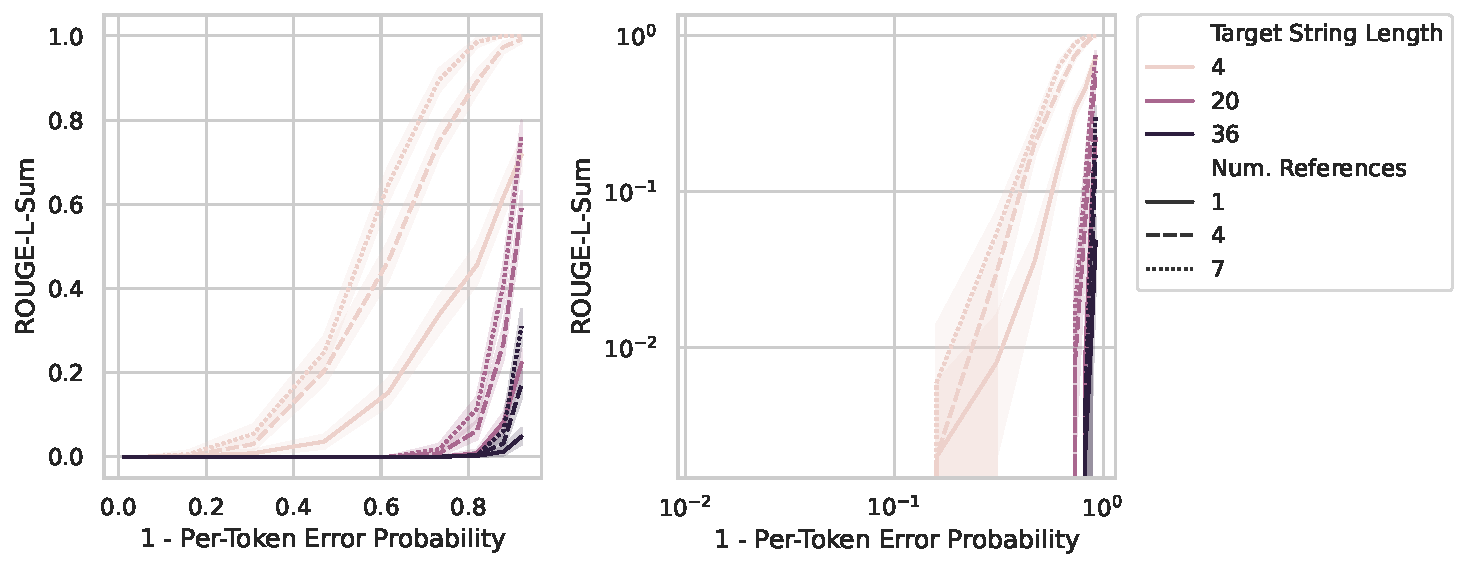
\includegraphics[width=0.95\textwidth]{figures/rouge_understanding/rougeLsum_vs_token_error_prob_scaling_simulation.pdf}
    \caption{\textbf{ROUGE-L-Sum is a sharp metric.} Simulations show that as the per-token error probability slightly increase (e.g. from 0.05 to 0.1), the ROUGE-L-Sum metric sharply falls.}
    \label{fig:app:metric_scaling:rougeLsum}
\end{figure}


Another BIG-Bench metric \cite{srivastava2022beyond} is ROUGE-L-Sum \cite{lin2004rouge}, a metric based on the longest common subsequence (LCS) between two sequences. Section 3.2 of \cite{lin2004rouge} gives the exact definition, but the key property is that ROUGE-L-Sum measures the ``union" LCS, which means ``stitching" together LCSs across the candidate and multiple references. As explained in the original paper: if the candidate sequence is $c = w_1 w_2 w_3 w_4 w_5$, and if there are two reference sequences $r_1 = w_1 w_2 w_6 w_7 w_8$ and $r_2 = w_1 w_3 w_8 w_9 w_5$, then $LCS(r_1, c) = w_1 w_2$ and $LCS(r_2, c) =w_1 w_3 w_5$, then the \textit{union} 
-LCS of $c, r_1, r_2$ is $w_1 w_2 w_3 w_5$, with length 4. Intuitively, this disproportionately benefits models with smaller error rates because their mistakes can be ``stitched" across multiple references; this is confirmed in simulation (Fig. \ref{fig:app:metric_scaling:rougeLsum}).


% \subsection{BLEU}
% \label{app:metric_scaling:bleu}


% \subsection{Emergence does not require on scaling laws: decreasing cross-entropy loss and stricter exact match is all you need }

% The goal of this section is to show that scaling laws are not necessary to create emergence and that many functional forms of the loss are valid as long as the form decreases as some other variable decreases -- say the number of parameters in the model.
% This typically holds in modern machine learning. 
% We do this by considering different functional forms of the cross entropy $CE(N)$, as a function of the number of parameters $N$, and show emergence, i.e. sharpness and unpredictability.
% We illustrate this by showing the programmer can exaggerate the sharpness (and therefore emergence) by implying increasing the exact number of tokens required to get correct in the accuracy, i.e. increasing $L$ in our notation.

% \subsubsection{Argument}

% Recall from section \ref{sec:alt_explanation} the accuracy requiring all $L$ tokens to be correct for a model of size $N$ as a function of cross-entropy $CE(N)$:

% \begin{equation*}
%     \text{Accuracy}(N) \approx p_N(\text{single token correct})^{\text{num. of tokens}} = \exp \Big(- CE(N) \Big)^L
% \end{equation*}

% We plot this equation using three functional forms for a decreasing cross-entropy loss in figure \ref{fig:decreasing_loss_leads_to_emergence_as_L_increases} for increasing values of $L$.
% These increasing values of $L$ induce a sharper -- therefore, seemingly more emergent curve when plotting the accuracy. 
% This means that if the programmer simply requires a stricter accuracy, he can make a perfectly smooth and predictable cross-entropy loss suddenly become sharp and unpredictable, i.e. ``emergent". 
% We show numerically it is independent of the functional form and instead that it only requires the cross-entropy to be decreasing and the accuracy metric to have some non-linear transformation that makes it sharper. 
% Therefore, if one had only tracked the cross-entropy loss instead, one could have had a smooth predictable curve for the models.
% This implies small-scale experimentation is still relevant, and we wish to highly that GPT-4 \cite{gpt4} small-scale experiment in conjunction with scaling loss. 
% We'd like to emphasize that changing the evaluation metric can suddenly induce emergence, and it is not an intrinsic property of the model. 

% %The goal will be to show that if $CE(N)$ decreases with different functional forms that $acc$ is emergent (either sharp or unpredictable).
% % TODO: sharp due to L
% % TODO: unpredictable due to constant and L

% \begin{figure}[htbp]
%   \centering
%   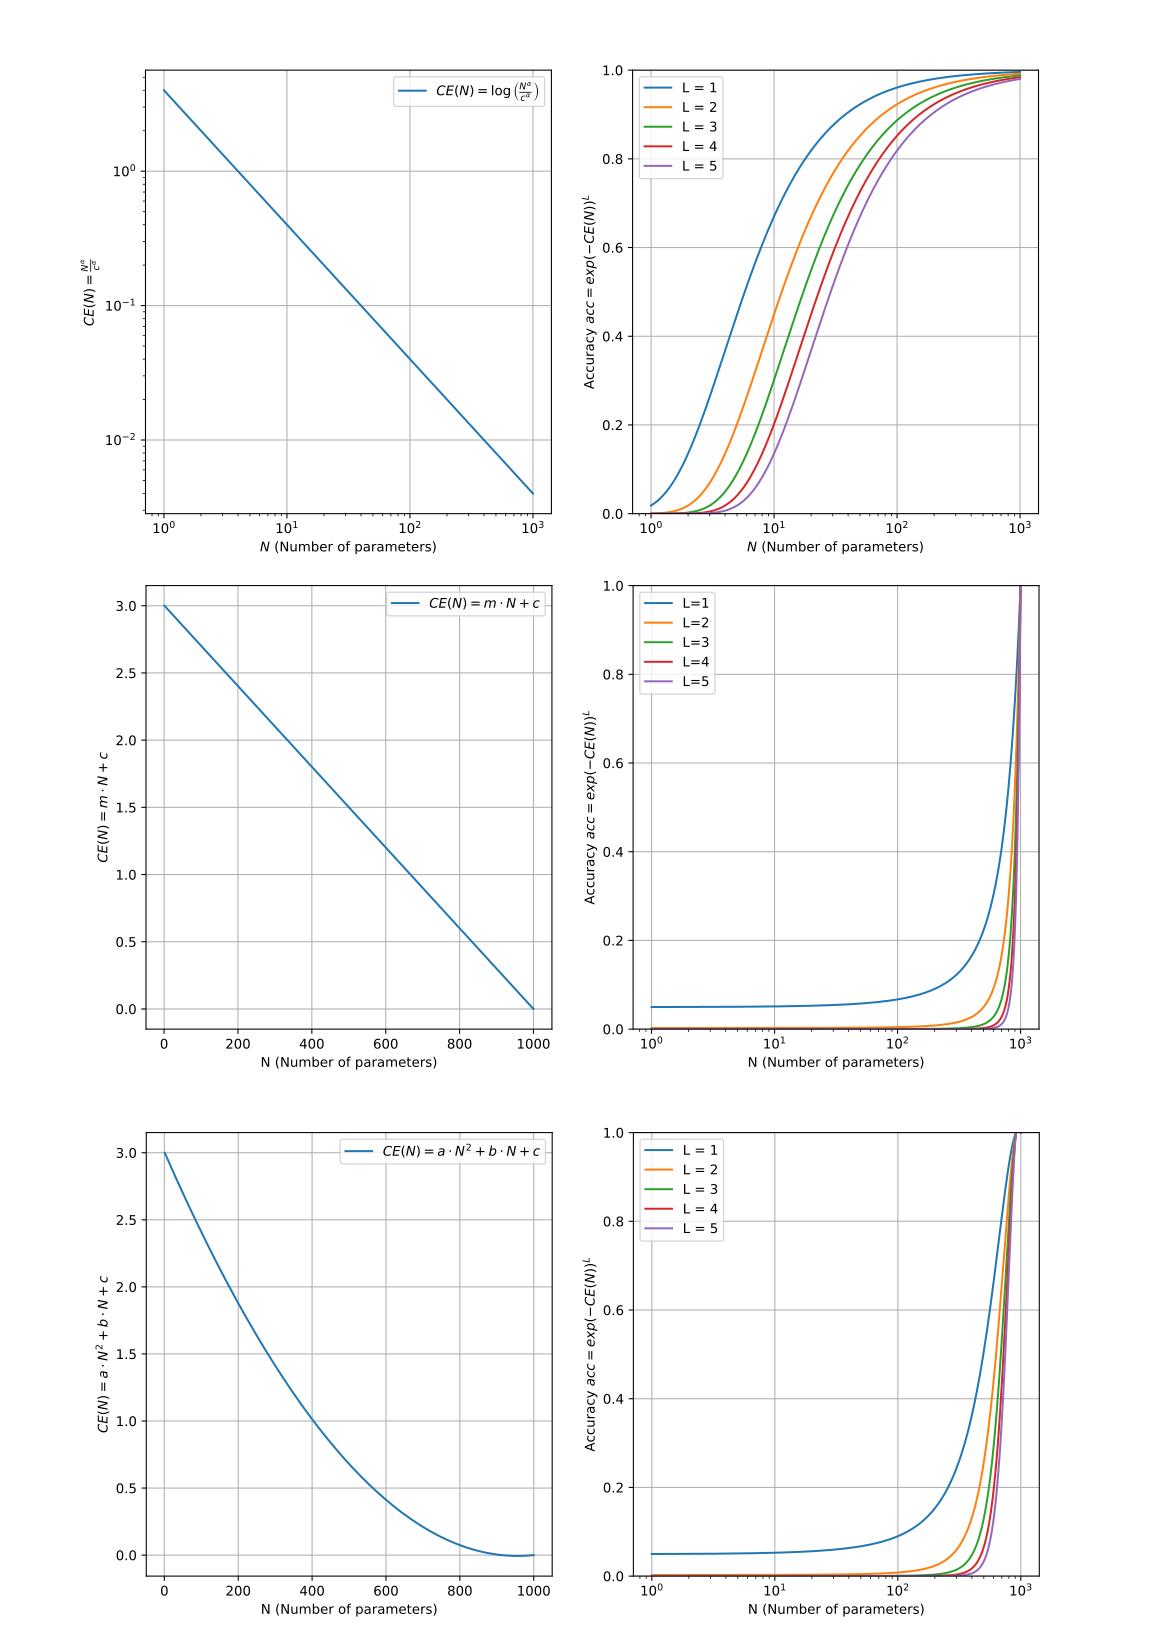
\includegraphics[width=0.8\textwidth]{figures/loss_decreasing_leads_to_emergence/decreasing_loss_leads_to_emergence_as_L_increases.png}
%   \caption{
%   \textbf{Emergence does not depend on scaling laws: any decreasing cross-entropy loss induces apparent emergence as L increases as you require more tokens to be exactly correct, i.e. L increases.}
%   The first row shows the same argument as in the main section, where a decreasing cross-entropy loss as a scaling law induces emergence as $L$ increases.
%   The second row shows the that apparent emergence is induced even when the cross-entropy loss decreases linearly.
%   The third row shows that the apparent emergence is induced when the cross-entropy loss decreases quadratically.
%   Emergence is amplified in this case especially by the increase in sharpness as more tokens are required to be correct. 
%   This means that simply changing the evaluation metric can suddenly induce emergence, and it is not an intrinsic property of the model. 
%   }
%   \label{fig:decreasing_loss_leads_to_emergence_as_L_increases}
% \end{figure}


\section{Inducing Emergent Abilities in Networks on Vision Tasks}
\label{app:sec:inducing_emergence_vision}

\subsection{Emergent Classification of MNIST Handwritten Digits by Convolutional Networks}

\begin{figure}
    \centering
    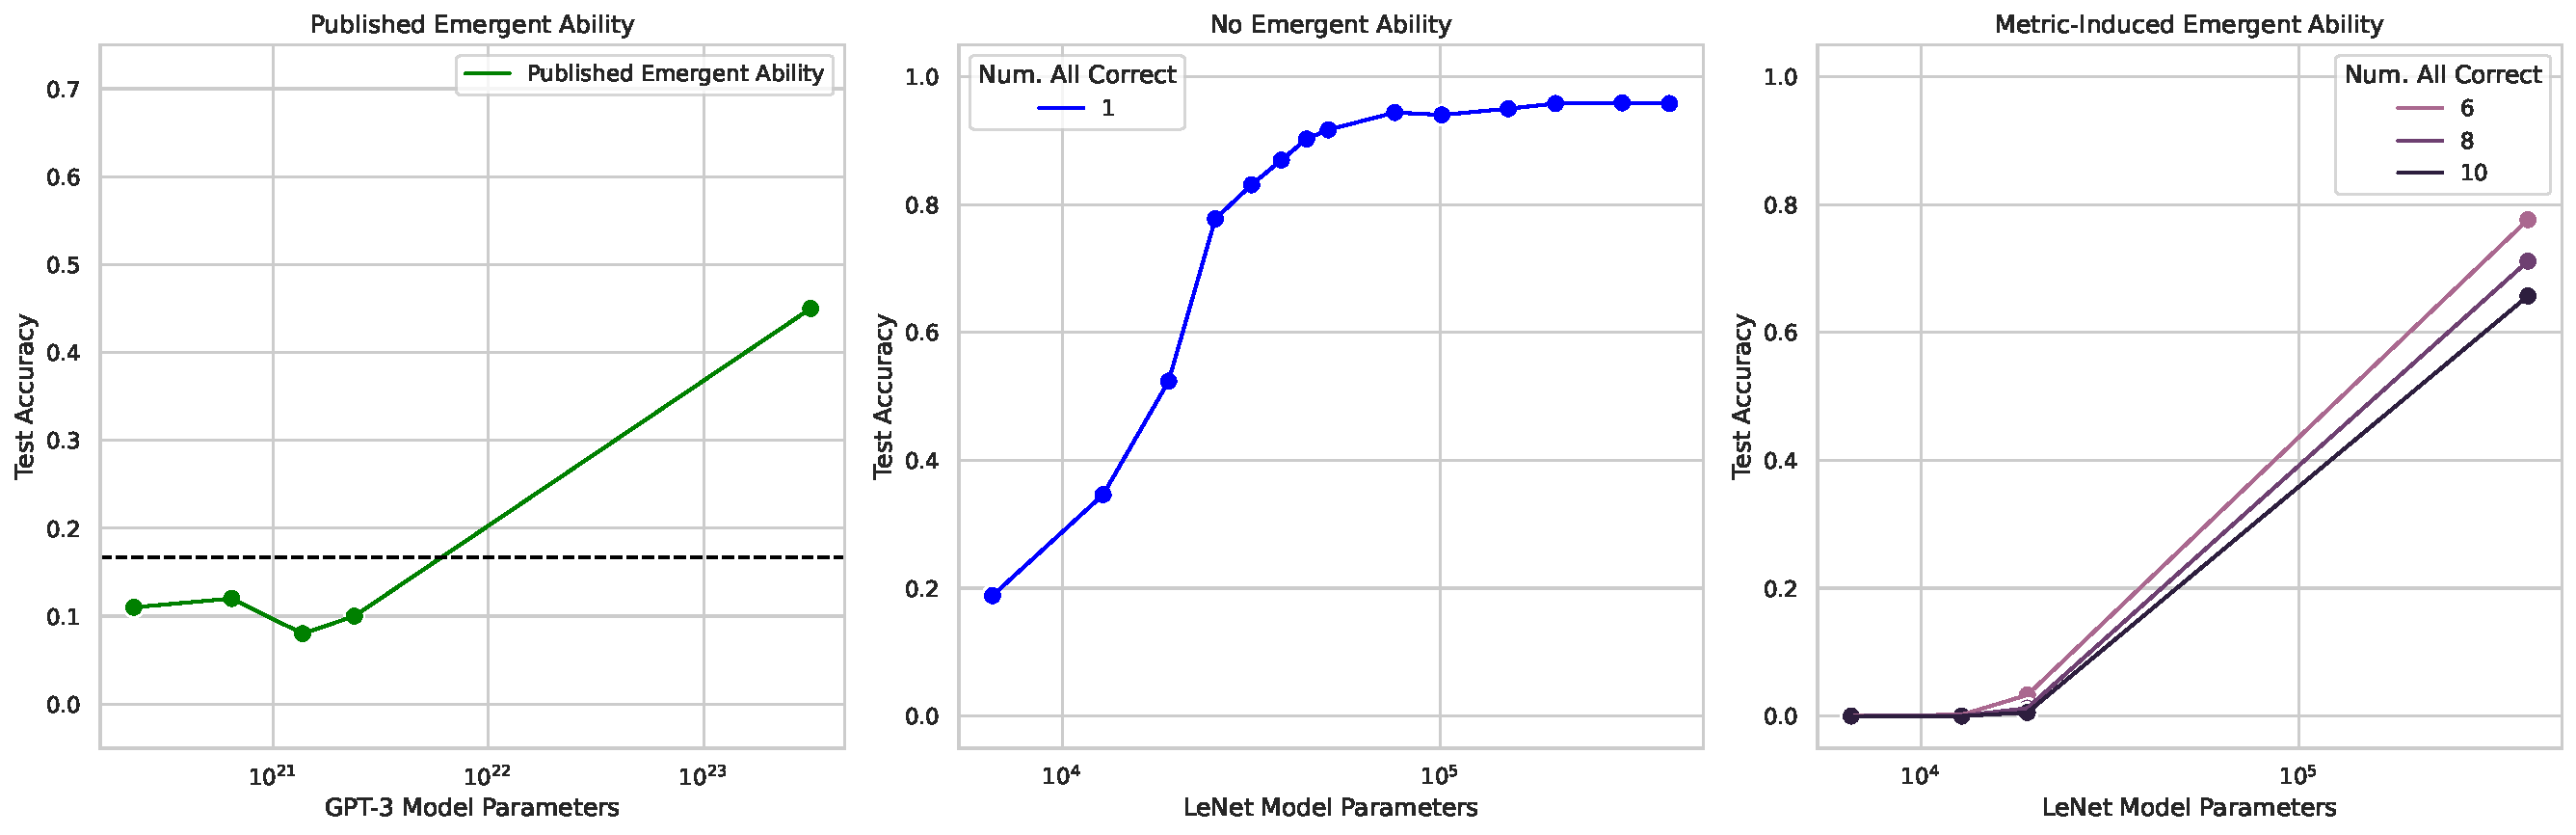
\includegraphics[width=\textwidth]{figures/vision/no_emergence_and_emergence_dataset=mnist.pdf}
    \caption{\textbf{Induced emergent MNIST classification ability in convolutional networks.} (A) A published emergent ability from the BIG-Bench Grounded Mappings task \cite{wei2022emergent}. (B) LeNet trained on MNIST \cite{lecun1998mnist} displays a predictable, commonplace sigmoidal increase in test accuracy as model parameters increase. (C) When accuracy is redefined as correctly classifying $K$ out of $K$ independent test data, this newly defined metric induces a seemingly unpredictable change.}
    \label{fig:vision_mnist}
\end{figure}

We begin by inducing an emergent classification ability in a LeNet convolutional neural network family \cite{lecun1998gradient}, trained on the MNIST handwritten digits dataset \cite{lecun1998mnist}.
This family displays smoothly increasing test accuracy as the number of parameters increase (Fig. \ref{fig:vision_mnist}B).
To emulate the accuracy metric used by emergence papers \cite{ganguli2022predictability, wei2022emergent, srivastava2022beyond}, we use \textit{subset accuracy}: 1 if the network classifies $K$ out of $K$ (independent) test data correctly, 0 otherwise.
Under this definition of accuracy, the model family displays an ``emergent" ability to correctly classify sets of MNIST digits as $K$ increases from $1$ to $5$, especially when combined with sparse sampling of model sizes (Fig. \ref{fig:vision_mnist}C).
This convolutional family's emergent classification ability qualitatively matches published emergent abilities, e.g., at the BIG-Bench Grounded Mappings task \cite{wei2022emergent} (Fig. \ref{fig:vision_mnist}A).

\end{document}